% ==============================================================================
\chapter{Semiconductor detectors}
\label{sec:SiliconTheory}
%==============================================================================    

Semiconductor materials have a great advantage in many radiation
detection applications. The main benefits are the high energy
resolution due to the large number of free charge carriers that are
created by a given incident radiation, their compact sizes, fast
timing, while the effective thickness can be adapted to the
requirements of the applications. Though, they show some limitations
for smaller sizes and their performance can degrade from radiation
induced damages. Among semiconductor materials, silicon detectors are
predominant for charged particle spectroscopy.

In this chapter, we will review the basic properties of semiconductor
material, charge generation in silicon and the transport of charge
carriers through drift and diffusion. Pixel detectors are studied
through pn-junctions. 

%% --------------------------------------------- %%
\section{Basic properties of semiconductor material}
Due to the periodic lattice of crystalline structure of semiconductor
material, electrons within the solid have allowed energy bands. The
energy of the electrons is confined to one of the energy bands and the
bands may be separated by gaps of forbidden
energies.\\ \cref{fig:energyBands} schematically illustrates the bands
in insulators, semiconductors and metals. In the \textit{valence
  band}, the electrons are bonded to specific lattice sites within the
crystal. The electrons in the \textit{conduction band} are free to
move through the crystal and contribute to the electrical
conductivity. The \textit{bandgap} (E\textsubscript{g}) separates the
valence from the conduction band and allows to classify wether the
material is a semiconductor, an insulator or a metal. In the absence
of thermal excitation, the valence band for the semiconductors and
insulators is completely full and the conduction band empty. Therefore
they are not electrically conductive. Metals are highly electrically
conductive since the fermi energy level (E\textsubscript{F}) lies in
the conduction band and the electrons are free to migrate through the
material even at very low temperatures. However, for insulators and
semiconductors the electrons must cross the bandgap to become
conductive. The bandgap for semiconductors ($\sim1\,\ev$) is much
lower than for insulators ($\sim5\,\ev$). If an electron in the
valence band gains enough thermal energy to cross the bandgap and
reach the conduction band, it leaves behind a vacancy (a hole) behind
in the valence band. The electron-hole pair can move under the
influence of an external electric field (electrons in the opposite
direction of the holes). This motion creates conductivity in the
material. This property is exploited in silicon detectors to detect
radiation and is developed more in the coming sections.




\begin{figure}[htbp]
  \centering
  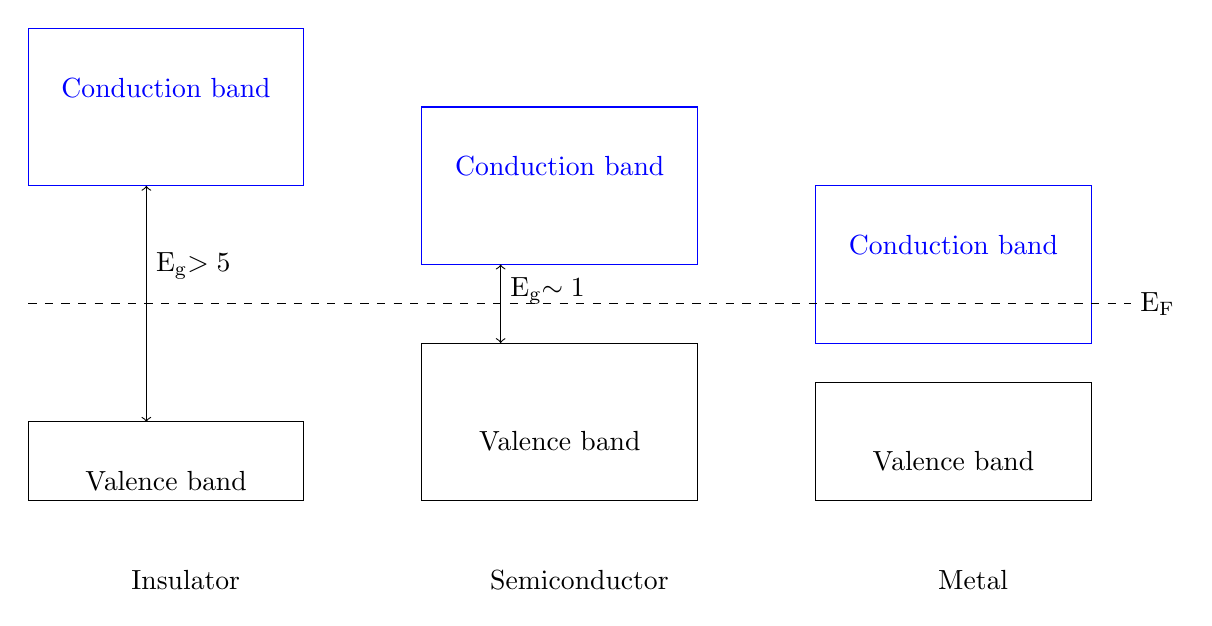
\begin{tikzpicture}
    \begin{scope} % Valence and conduction bands
      %  ----- insulator ----- %
        \draw (0, 1) rectangle node[below] {Valence band}  ++ (3.5, 1);
        \draw[blue] (0, 5) rectangle node[above] {Conduction band} ++ (3.5, 2);
        \node at (2, 0) {Insulator};

        % ----- Semiconductor ----- %
        \draw (5, 1) rectangle node[below] {Valence band}  ++ (3.5, 2);
        \draw[blue] (5, 4) rectangle node[above] {Conduction band} ++ (3.5, 2);
        \node at (7, 0) {Semiconductor};

        % ----- Metal ----- %
        \draw (10, 1) rectangle node[below] {Valence band}  ++ (3.5, 1.5);
        \draw[blue] (10, 3) rectangle node[above] {Conduction band} ++ (3.5, 2);
        \node at (12, 0) {Metal};
    \end{scope}


    \begin{scope} % Energy levels
        \draw[dashed] (0, 3.5) -- (14, 3.5) node[right] {E\textsubscript{F}};
        \draw[arrows=<->](1.5, 2)--(1.5, 5) node [pos=0.66,right] {E\textsubscript{g}$>5\,\ev$};
        \draw[arrows=<->](6, 3)--(6, 4) node [pos=0.66,right] {E\textsubscript{g}$\sim1\,\ev$};
    \end{scope}

  \end{tikzpicture}
  \caption{Illustation of the band structures for electron energies in
  insulators, semiconductors and metals. E\textsubscript{F} represents the Fermi energy level and E\textsubscript{g} the bandgap.}  
  \label{fig:energyBands}
\end{figure}

%% --------------------------------------------- %%
\subsection{Silicon}
\label{sec:silicon}

In semiconductors, the excitation energy is defined by the periodicity
of the crystal lattice. Silicon is a semiconductor with a
\textit{diamond} lattice as illustrated in
\cref{fig:SiliconDiamondLattice}. The dimension $a$ is the lattice
constant and is \SI{5.34}{\angstrom} in silicon.


\begin{figure}[htbp]
  \centering
  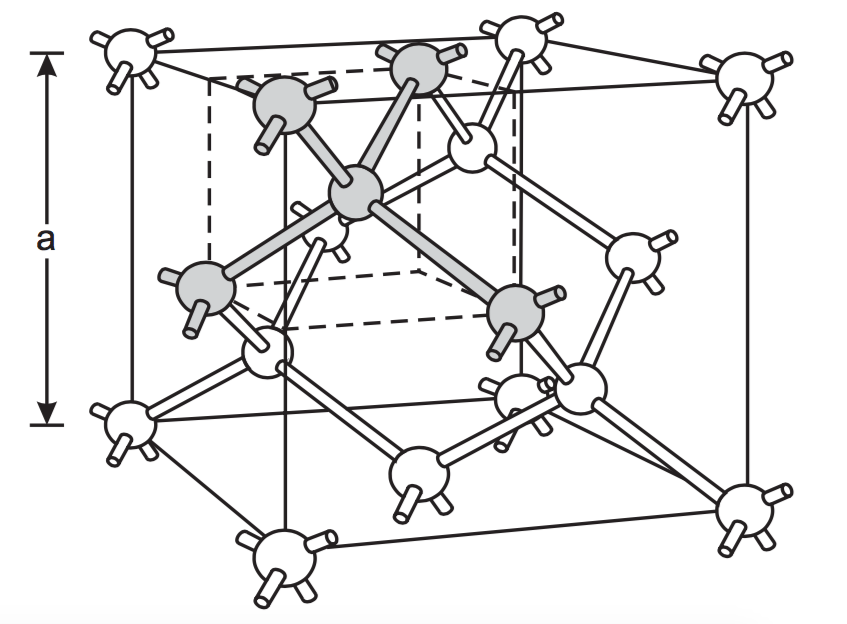
\includegraphics[width=0.5\textwidth]{figures/ChargeSharing/SiliconDiamondLattice.png}
  \caption{Lattice structure of silicon. The building block of the
    lattice is formed by a central atom bonded to four equidistant
    neighbours as shown in shaded
    gray. From~\cite{Spieler2005}.}\label{fig:SiliconDiamondLattice}
\end{figure}

In the periodic table, silicon is a group four element as it has four
valence electrons and which combine with four neighbours to build
covalent bonds and close the outer shell.  At 0~K, no electrical
conduction is possible since all the electrons fill completely the
valence band. An incident radiation can break a bond and excite an
electron into the conduction band. This leaves a \textit{hole} or a
vacant state in the valence band and the electron can freely move in
the conduction band. The hole can also move in the valance band by the
indirect mechanism where an electron from a neighbouring atom fills it
and creates another hole.

An external electric field can direct the motion of the electrons and
holes created. Holes are treated as positive charge carriers. 

In silicon, the ionisation energy or the average energy deposition
required to produce an electron-hole pair is $3.6\,\ev$.

%% --------------------------------------------- %%
\subsection{Doping}
\label{sec:doping}

By introducing special impurities, the conductivity of semiconductors
can be controlled. Typical concentration ranges between
$10^{12}-10^{18}\,\inversecmcubic$. In semiconductors, the
conductivity comes from either electrons (n-type) or holes (p-type).

In \textit{n-type doping}, a silicon atom is replaced with an atom
having five valence electrons, for example phosphorus. This creates an
excess in electrons into the lattice and is called a donor. The donor
electron is lightly bound to the impurity atom. As a consequence, the
ionisation probability is increased and mobile electrons are
introduced into the conduction band.

In \textit{p-type doping}, by introducing a group three atom into the
silicon lattice such as the boron, one impurity valence electron is
left. This type of dopant is called an acceptor: the dopant borrows an
electron from a neighbouring atom and the holes can move freely
throughout the crystal.
 
%% --------------------------------------------- %%
\section{Charge generation and recombination in silicon}
\label{sec:chargeInSi}

Previously, we have reviewed the basic properties of semiconductor
material with a focus on silicon. The electron-hole generation is also
introduced. In this section, we focus on the amount of charge
generated due to an incident radiation.

\subsection{Bethe-Bloch formula}
In silicon, free charge careers are generated due to thermal effects
and lead to leakage current. A current is also generated due to the
interaction of charged particles with silicon and can be
detected. Part of the absorbed energy generates electron-hole pairs
through scattering processes with the shell electrons of silicon and
can be collected by the readout electronics. The number of
electron-hole pairs produced, as well as the total energy loss of the
particle in the detector, are stochastic quantities.

The energy loss along the particle track is described by the
Bethe-Bloch formula~\cite{Beringer:1900zz}:

\begin{equation}
  - \braket{{dE}\over{dx}} = 4 \pi N_A r_{e}^2 m_e c^2 z^2 \frac{Z}{A}  \frac{1}{\beta^2} \left[ \frac{1}{2} \ln{\frac{2 m_e c^2 \beta^2 \gamma^2 T_{max}}{I^2}} - \beta^2 - \frac{\delta\left(\beta\gamma\right)}{2}\right]\; ,
  \label{eq:BetheBloch}
\end{equation}

where $N_A$ is the Avogadro's number, $r_e$ the classical electron
radius, $m_ec^2$ the rest energy of the electron, $z$ is the charge of
the traversing particle, $Z$ the atomic number, $A$ the atomic mass of
the absorption medium, $\beta={v \over c}$,
$\gamma=1/\sqrt{1-\beta^2}$, $I$ the mean excitation energy, $T_{max}$
the maximum kinetic energy that a particle can transfer to a shell
electron and $\delta\left(\beta\gamma\right)$ the density effect
correction to ionisation energy loss. Relativistic particles with an
energy loss near the minimum of the Bethe-Bloch formula are considered
as minimum ionising particles (MIPs).

\subsection{Energy-loss spectrum in silicon}
\label{sec:SiliconEnergyLossSpectrum}
Ionisation is also subject to statistical fluctuations and
\cref{eq:BetheBloch} gives its average value. It can be described by a
probability density function called \textit{straggling function} and
characterised by the most probable energy loss ($\Delta_{p}$) and
full-width-at-half-maximum ($w$). \cref{fig:LandauDistribution} shows
examples of this distribution in thin sensors. If a particle is not
stopped in the sensor, the energy deposition varies around the peak of
the distribution with a large tail for high signals. The main reason
for the highly-skewed energy-loss distribution is the manifestation of
$\delta$-rays which happens when electrons acquire enough energy by
interaction and themselves become ionising particles. The
$\delta$-rays not only make the average value of the energy-loss
higher than the most probable value ($\Delta_{p}$) of the
distribution, but also create big clusters and thus degrade the
spatial resolution of the detector. This is the reason why the Bethe
equation (c.f. \cref{eq:BetheBloch}) is ill-defined experimentally and
not used for applications where the energy loss for single particles
is described.

The fluctuations around $\Delta_{p}$ increase for thinner sensors and
should be taken into account for the design of the dynamic range of
the readout electronics.


\begin{figure}[htbp]
  \centering
  \includegraphics[width=0.7\textwidth, page=14, trim = 50mm 160mm
    40mm 20mm, clip]{Articles/rpp2009-rev-passage-particles-matter.pdf}
  \caption{Straggling function in silicon for 500 MeV pions,
    normalized to unity at the most probable value $\Delta_{p}$. $w$
    is the full-width-at-half-maximum~\cite{Beringer:1900zz}.}
  \label{fig:LandauDistribution}
\end{figure}

In literature, several approaches address the calculation of the
straggling functions. The Landau and the Bichsel models, two of the
most relevant models, are described in \cref{sec:landau,sec:bichsel}. 

The probability of the occurrence of collisions and the probability
for a particular energy loss $E$ are considered for the calculation of
the straggling functions. To obtain correct straggling functions, the
accurate determination of the collision cross section as function of
energy loss, $\sigma(E)$, is necessary.

\subsection{The Landau distribution}\label{sec:landau}
The most commonly used model in experiments, is a Landau distribution
convoluted with a Gaussian. The most probable value $\Delta_p$ of the
distribution is given by the Landau-Vavilov
method~\cite{Landau:1944if,Vavilov:1957zz}:

\begin{equation}
  \Delta_p=\xi \left[\text{ln}{{2mc^2\beta^2\gamma^2}\over{I}}+\text{ln}{\xi \over I}+0.200-\beta^2-\delta\left(\beta\gamma\right) \right] \; ,
  \label{eq:LandauVavilovMPV}
\end{equation}

where $\xi=(K/2)\braket{Z/A}(x/\beta^2)$~\mev for a detector of
moderate thickness $x$ in g~\inversecmsquared. All the other
parameters are similar to the ones described for \cref{eq:BetheBloch}.

Though the Landau-Vavilov calculation does not describe correctly the
width of the energy distribution for thin silicon sensors. For thick
material, the width of the distribution is $4\xi$.

For $\gamma\gg100$, \cref{eq:LandauVavilovMPV} is simplified to~\cite{Bichsel}

\begin{equation}
  \textsubscript{L}\Delta_{p} (\kev)=t \left(0.1791+0.01782 \ln\left(t\right)\right) \; ,
  \label{eq:LandauVavilovMPV_simplified}
\end{equation}

where $t$ (in \micron) is the thickness of the silicon.

When the Landau distribution is combined with a Gaussian, $\Delta_ p$
increases and gives better agreement with data.

\subsection{The Bichsel model}\label{sec:bichsel}
The Bichsel model~\cite{Bichsel} takes into account the binding of
atomic electrons to find a better agreement between data and
theory. In this model, experimental and theoretical data for
dielectric functions, x-ray absorption coefficients and generalised
oscillator strengths are used to reproduce accurately the observed
energy loss spectrum over a wide range of incident particle velocities
and silicon thicknesses, including very thin silicon sensors. But no
analytical description of the straggling function is provided.

Bichsel provides an approximation of $\Delta_{p}$ and $w$ (in \ev) as
function of the thickness $t$ (in $\micron$) of silicon detectors for
particles with charge $\pm1e$ and $\beta\gamma>500$ as listed in
\cref{eq:MPV1,eq:MPV2,eq:FWHM}:

\begin{itemize}
\item For $13<t<110$ [\micron]:
  \begin{equation}
    \Delta_{p}=t \cdot \left(100.6+35.35 \cdot \ln(t) \right)\; ,
    \label{eq:MPV1}
  \end{equation}
\item For $110<t<3000$ [\micron]:
  \begin{equation}
    \Delta_{p}=t \cdot \left(190+16.3 \cdot \ln(t) \right)\; ,
    \label{eq:MPV2}
  \end{equation}
\item For $30<t<260$ [\micron]:
  \begin{equation}
    w=t \cdot \left(259.6-28.41 \cdot \ln(t) \right).
    \label{eq:FWHM}
  \end{equation}
\item For $260<t<2560$ [\micron]:
  \begin{equation}
    w=71.3 t \left( 1+ 39.4/t^{0.8} \right)
    \label{eq:FWHM2}
  \end{equation}
\end{itemize}

\cref{tab:EdepForDifferentThickness} summarises the $\Delta_{p}$ and
$w$ for detectors thicknesses at our disposal and tested at test beams
with the results presented in the following chapters.

\begin{table}[htbp]
  \centering
  \caption{Calculated $\Delta_{p}$ and $w$ for silicon sensors with
    various thicknesses using
    \cref{eq:MPV1,eq:MPV2,eq:FWHM,eq:FWHM2}.}
  \label{tab:EdepForDifferentThickness}
  \begin{tabular}{c c c c}
    \toprule
    Thickness [\micron] &  $\Delta_{p}$ [\kev] & $w$ [\kev] & $\Delta_{p} / w$ \\ 
    \midrule
    50 & 11.9 & 7.42 & 1.6      \\
    100 & 26.34 & 12.88 & 2.045 \\
    150 & 40.75 & 17.59 & 2.32  \\
    %%200 & 55.27 & 21.82 & 2.53  \\
    300 & 84.89 & 30.18 & 2.8 \\
    \bottomrule
  \end{tabular}
\end{table}

\subsection{Multiple scattering}

In addition to energy loss, when a particle goes through the detector,
its trajectory is deflected by small-angle scatters. The deflection is
mainly due to the Coulomb interaction of the charged particle with the
nuclei. The strong interaction has also a contribution for
hadrons. When leaving the detector, the scattering angle of the
particle follows a Gaussian distribution with an RMS given
by~\cite{Lynch:1990sq}:

\begin{equation}
  \theta\textsuperscript{RMS}={{13.6\,\mev}\over{\beta p c}} z
\sqrt{x \over X_0} \left[1+0.038\ln{\left(x \over X_0 \right)}\right],
  \label{eq:multipleScattering}
\end{equation}

where the angle $\theta$ is in radians, the particle momentum $p$ in
\mev, $z$ the charge number of the particle and $x/X_0$ the thickness of
the absorption medium in units of the radiation length.

In high-energy physics applications, the material budget of pixel
detectors is minimised in order to have the smallest scattering angles
possible.

%% --------------------------------------------- %%
%% \subsection{\textsc{Geant4}}\label{sec:Silicon_Geant4}
%% --------------------------------------------- %%
\section{Silicon device physics and properties}


In this section, we review the motion of the charge carriers in
silicon. First the motion in an intrinsic silicon is studied. Then, a
pn-junction is described and the motion of charge carriers in silicon
detectors is sketched.

\subsection{Transport of charge carriers}
In silicon detectors, the movement of the charge carriers (holes and
electrons) leads to signal pulses in the electrical contacts which can
be detected by the readout electronics.  In the absence of any
external electric field, free charge carriers move randomly and are
scattered due to their collisions with the crystal lattice or other
impurities. On average, in equilibrium conditions, the traveled
distance averaged over charges is zero. In addition to the statistical
movement, two other mechanisms can affect the transport of charge
carriers: diffusion (due to a gradient in concentration) and drift (in
the presence of an external electric field).

The diffusion implies that a carrier is more probable to move from a
high-concentration region to a low-concentration region. The diffusion
current per unit area is given by~\cite{Rossi:976471}:

\begin{equation}
  \begin{aligned}
    J_{n, diff}=-{kT \over e} \mu_n \nabla n \qquad \textnormal{for electrons}
    \; , \\
    J_{p, diff}={kT \over e} \mu_p \nabla p \qquad \textnormal{for holes}
    \; , 
  \end{aligned}
  \label{eq:diffusionCurrent}
\end{equation}
where $k$ is the Boltzmann constant, $T$ the absolute temperature, $e$ the
elementary charge, $\mu$ the mobility of the charge carriers, $\nabla
n$ and $\nabla p$ are the gradients of the electron and hole
concentrations.

Charge carriers are accelerated between two random collisions in the
presence of an external electric field in the direction of the field
and leads to and average drift velocity given by~\cite{Rossi:976471}:

\begin{equation}
  \begin{aligned}
    v_{n}=-\mu_n \textbf{E} \qquad \textnormal{for electrons}
    \; , \\
    v_{p}=\mu_p \textbf{E} \qquad \textnormal{for holes}
    \; , 
  \end{aligned}
  \label{eq:driftVelocity}
\end{equation}
where $v$ is the average drift velocity, $\textbf{E}$ the electric
field and $\mu$ the mobility of the charge carriers. The mobility is a
function of the electric field. For higher electric fields the charge
carriers gain more acceleration and the number of collisions per unit
time increases. This leads to a saturation of the drift velocity
$v_s$. The mobility dependence on the electric field is described by~\cite{Jacoboni197777}:
\begin{equation}
  \mu=\frac{v_{s}/E_{c}}{\left[1+(E/E_{c})^{\beta}\right]^{1/\beta}}\; ,
  \label{eq:mobility}
\end{equation}

where the parameters are described in \cref{tab:mobility_parameters}.

\begin{table}[htbp]
  \centering
  \caption{Parameters for the mobility as described in
    \cref{eq:mobility} with T the absolute temperature and E the
    absolute electric field.}
  \label{tab:mobility_parameters}
  \begin{tabular}{c c c c}
    \toprule
    Parameter & Electrons & Holes & unit \\
    \midrule
    $v_s$ & 1.53 $\times$ $10^9$ $\times$ T\textsuperscript{-0.87} &
1.62 $\times$ $10^8$ $\times$ T\textsuperscript{-0.52} & cm/s \\ 
    $E_c$ & 1.01 $\times$ T\textsuperscript{1.55} & 1.24 $\times$ T\textsuperscript{1.68} & V/cm \\ 
    $\beta$ & 2.57 $\times$ $10^{-2}$ $\times$ T\textsuperscript{0.66} & 0.46 $\times$ T\textsuperscript{0.17} & -\\
    \bottomrule
  \end{tabular}
\end{table}

\cref{fig:Mobility_electron_holes} shows the mobility for electrons
and holes as a function of the electric field. For a low electric
field, the mobility for intrinsic silicon at 300~K is:
\begin{equation*}
  \begin{aligned}
    \mu_n=1415 \pm 46 \qquad \textnormal{\cmsquared/(Vs)} \; , \\
    \mu_p=480 \pm 17 \qquad \textnormal{\cmsquared/(Vs)} \; .
  \end{aligned}
\end{equation*}

\begin{figure}[htbp]
  \centering
  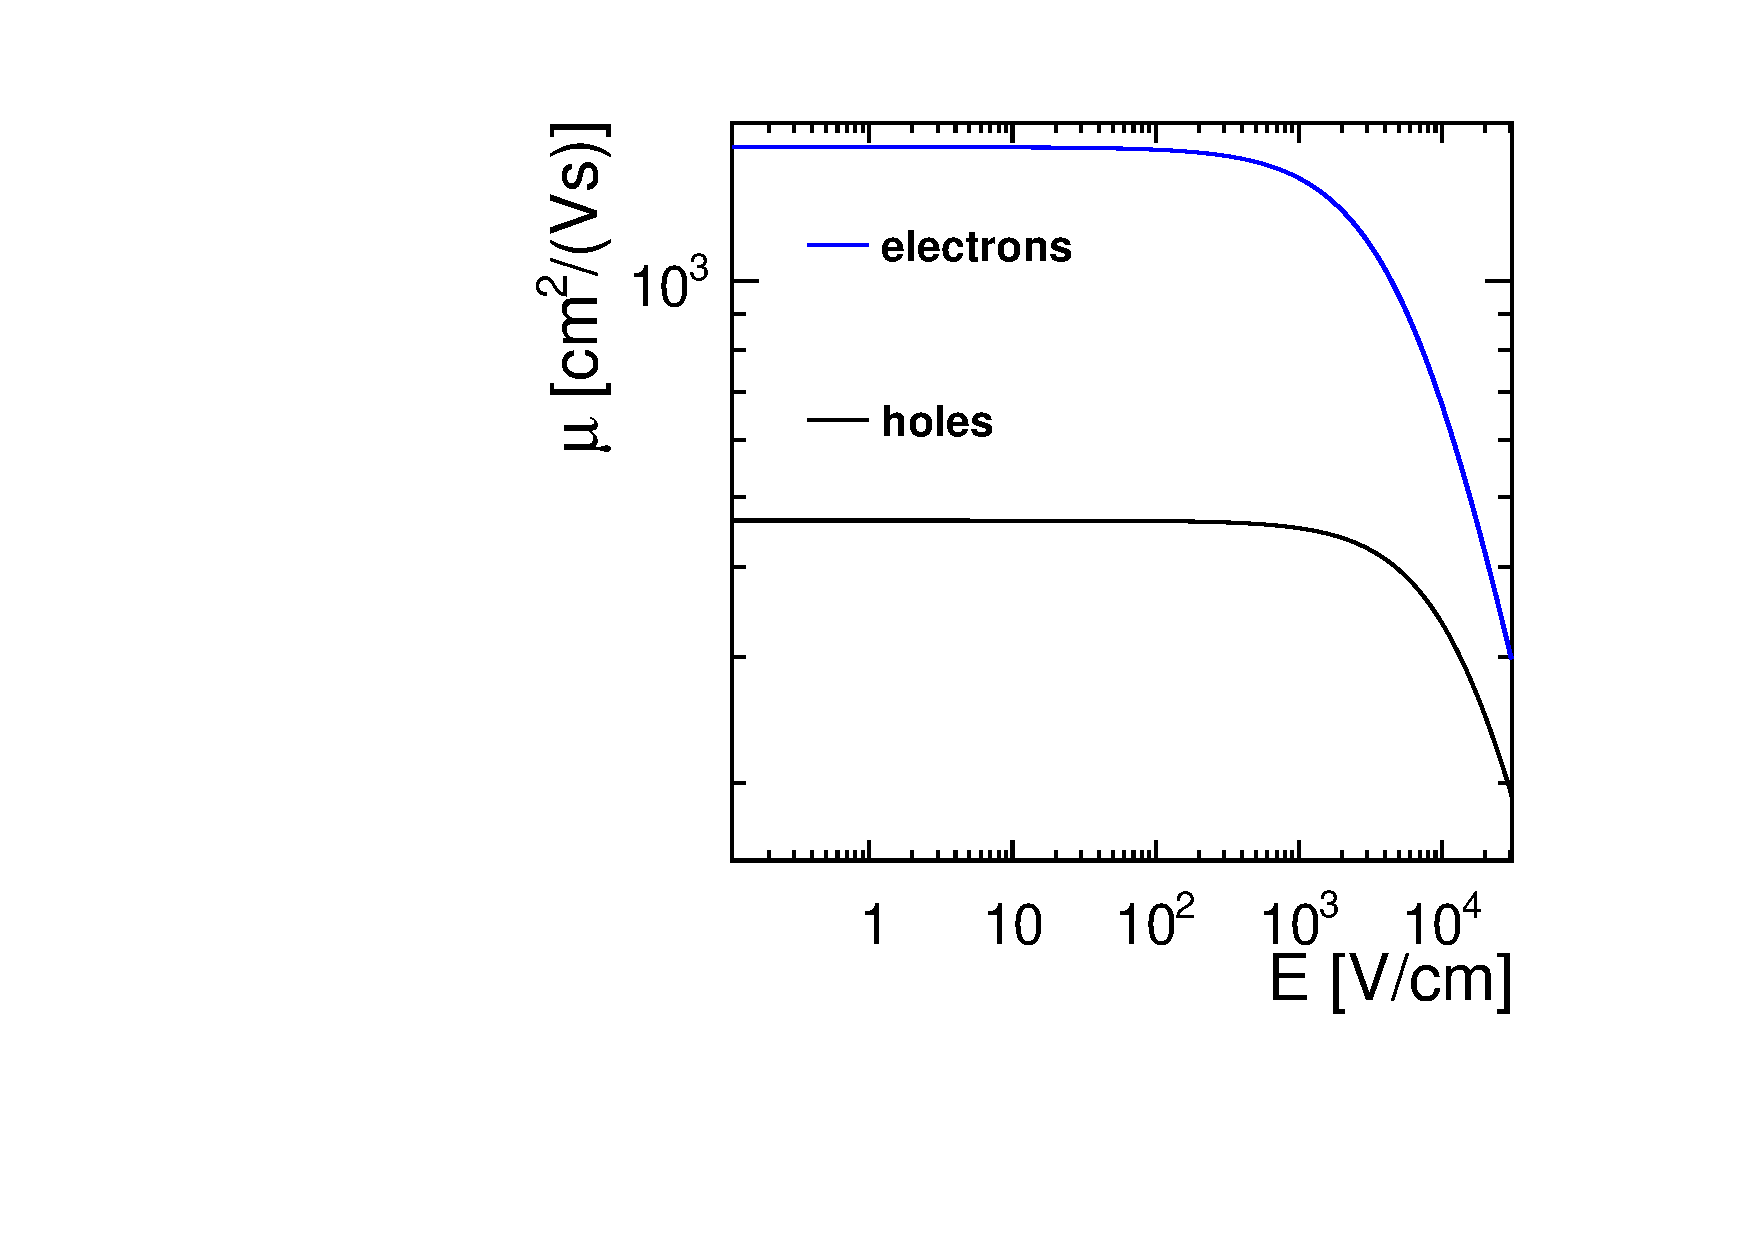
\includegraphics[width=0.5\textwidth]{figures/ChargeSharing/Mobility_electron_holes.pdf}
  \caption{Mobility for electrons and holes as a function of an
    applied electric field calculated with the \cref{eq:mobility}.}
  \label{fig:Mobility_electron_holes}
\end{figure}


Holes are three times less mobile than electrons which make them more
likely to be trapped in an irradiated material.

%% --------------------------------------------- %%
%\section{Pixel detectors: pn-junction}

% Silicon sensors are made of reversely biased pn-junctions. The
% electric field due to the bias voltage allows the charge carriers to
% drift towards the readout chip and also to suppress the leakage
% current.

\subsection{pn-junction in thermal equilibrium}

By joining a p-type with an n-type material, a pn-junction is
obtained. The p and n-type regions are electrically neutral. Due to
thermal diffusion, the holes and the electrons are driven across the
junction. This implies that electrons move from the n-type material to
the p-regions leaving a positive net charge in n-regions, while the
p-type region gets negatively charged. A potential is built up when
the electrons diffuse to the p-region. This potential limits the
diffusion depth when it exceeds the available energy for thermal
diffusion and is called the built-in potential $V_{bi}$ between the p
and n-regions. The built-in potential depends logarithmically on the
doping levels~\cite{Spieler2005}:

\begin{equation}
  V_{bi}= {{kT}\over e} \text{log}\left({N_a N_d} \over {n_i^2} \right)\; ,
  \label{eq:Built_in_potential}
\end{equation}

where $N_a$ and $N_d$ are the acceptor and donor concentrations and
$n_i$ is the intrinsic silicon carrier concentration. For a typical
detector diode $V_{bi}\approx0.5$~V.

The diffusion of the holes and electrons across the junction to the
oppositely-doped regions, leads to a region free of mobile carriers
called the depletion region. As seen previously, $V_{bi}$ limits the
diffusion depth and therefore the width of the depletion region.

Applying an external potential breaks down the thermal equilibrium. By
applying a reverse bias potential, i.e. negative potential to the
p-region and positive potential to the n-region, the potential barrier
and the depletion width are increased.

Under a forward bias on the pn-junction, the diode current increases
rapidly with the voltage. But a reverse bias causes a quick
saturation of the current flow within the junction and the pn-diode
can be used as a rectifier. This property is used for the detection of
radiation in silicon detectors as described in the next section.

\subsection{reverse-biased pn-junction}

The reverse-biased pn-junction is crucial in detection of radiation in
silicon detectors as it increases the depletion width. This forms a
capacitor empty of charge carriers where the undepleted p and
n-regions are the electrodes and the depletion region is the
dielectric. The electric field in the depletion region attracts the
mobile carriers to the electrodes.  The electric field due to the bias
voltage allows the charge carriers to drift towards the readout chip
and also to suppress the leakage current which can be an important
source of noise.

Here, we derive the depletion width, the electric field distribution,
the drift and the diffusion within a pn-junction reverse-biased at a
voltage of $V_B$.

The potential $\varphi$ at each point is described by Poisson's
equation~\cite{Knoll2010}:

\begin{equation}
  \nabla^{2}  \varphi=-{\rho \over \epsilon}\; ,
  \label{eq:poisson}
\end{equation}

where $\epsilon$ is the dielectric constant of the medium and $\rho$
the net charge density. The electric field E due to the electric
potential is obtained by:

\begin{equation}
E=-\text{grad }\varphi \; .
\label{eq:Efield}
\end{equation}


To simplify, we assume an abrupt junction where the charge densities
on the p and n-regions illustrated in \cref{fig:chargeDensity} and
given by:
\begin{equation}
  \rho(z)= 
  \begin{cases} 
    eN_{d}, & \mbox{if } 0\leq z < z_{n}\\ 
    -eN_{a}, & \mbox{if } z_{p}\leq z < 0 
  \end{cases} 
  \; .
\label{eq:chargeDensity}
\end{equation}

\begin{figure}[htbp]
  \centering
  \begin{tikzpicture}[node distance = 2.5cm, auto]
    \begin{scope}[x={(image.south east)},y={(image.north west)}]

      \draw[black, thick, ->] (0.5, 0.1) -- (0.5, 0.9); 
      \node[above, color=black] at (0.5, 0.9) {$\rho$};
      \draw[black, thick, ->] (0.1, 0.5) -- (0.9, 0.5);
      \node[right, color=black] at (0.9, 0.5) {Depth (z)};
      \node[left, color=black] at (0.5, 0.6) {e$N_d$};
      \node[below, color=black] at (0.8, 0.5) {$z_n$};

      \node[above, color=black] at (0.3, 0.5) {$z_p$};
      \node[right, color=black] at (0.5, 0.2) {-e$N_a$};
      
      \draw[black, thick, dashed] (0.5, 0.6) -- (0.8, 0.6); 
      \draw[black, thick, dashed] (0.8, 0.6) -- (0.8, 0.5);
 
      \draw[black, thick, dashed] (0.3, 0.5) -- (0.3, 0.2);
      \draw[black, thick, dashed] (0.5, 0.2) -- (0.3, 0.2);

      % \draw[help lines,xstep=.1,ystep=.1] (0, 0) grid (1,1);
      % \foreach \x in {0,1,...,9} { \node [anchor=north] at (\x/10,0) {0.\x}; }
      % \foreach \y in {0,1,...,9} { \node [anchor=east] at (0,\y/10) {0.\y}; }

    \end{scope}
  \end{tikzpicture}
  \caption{Charge density distribution for a simplified pn-junction.}
  \label{fig:chargeDensity}
\end{figure}



In one dimension, Poisson's equation is simplified to:
\begin{equation}
{{d^{2}  \varphi(z)} \over {dz^{2}}}=-{\rho(z) \over \epsilon}\; .
\label{eq:poisson1D}
\end{equation}

First, considering the n-side, the first and second integrations of the Poisson equation give:
\begin{equation}
    {{d\phi(z)} \over {dz}}=-{{eN_{d}} \over \epsilon} (z-z_{n}) 
    \; ,
    \label{eq:PoissonIntegration1}
  \end{equation}

\begin{equation}
  \phi(z)=-{{eN_{d}} \over \epsilon} {z^{2} \over 2}+{{eN_{d}zz_{n}}\over \epsilon}+Vj
  \; ,
  \label{eq:PoissonIntegration2}
\end{equation}

where $V_j$ is the potential at the interface where the n- and the p-sides join. At the boundary of the depletion region $z=z_{n}$:

\begin{equation}
  \phi(z_{n})=V_{B}={{eN_{d}z_{n}^{2}} \over \epsilon}+V_j 
  \; ,
  \label{eq:BounderyPotential}
\end{equation}

where $V_B$ is the reverse bias voltage. In the p-region,

\begin{equation}
  V_j={{eN_az_p^2} \over {2\epsilon}}
  \; .
\end{equation}

The total potential is given by:

\begin{equation}
V_b={{e} \over {2 \epsilon}}(N_dz_n^2+N_az_p^2)
  \; .
\end{equation}

Since the overall charge neutrality is maintained,
\begin{equation}
N_d z_n=N_a z_p
  \; ,
\end{equation}

the reverse bias potential can be expressed as:

\begin{equation}
V_b={e \over {2\epsilon}}\left(1+{N_a \over N_d}\right) N_a z_p^2={e \over {2\epsilon}}\left(1+{N_d \over N_a}\right) N_d z_n^2
  \; .
\end{equation}

The depletion widths on the n- and p-sides of the junction are

\begin{equation}
  \begin{multlined}
z_n=\sqrt{{2 \epsilon V_b} \over {eN_d(1+N_d/N_a)}} \\
z_p=\sqrt{{2 \epsilon V_b} \over {eN_a(1+N_a/N_d)}} 
\; .
\end{multlined}
\end{equation}

The total depletion width is 

\begin{equation}
W=z_n+z_p=\sqrt{{2 \epsilon V_b \left(N_a+N_d\right)} \over {eN_aN_d} }
\; .
\end{equation}

Considering an asymmetrical junction with $N_d \ll N_a$ for which the
junction potential is equal to the potential of the p-contact:

\begin{equation}
V_j=\left(N_d \over N_a\right) {V_b \over \left(  1+N_d/N_a \right)} \stackrel{N_d \ll N_a}{\approx} {N_d \over N_a}V_b
\; .
\end{equation}


For a pixel detector with asymmetric junction with a highly doped
surface $N_c$ concentration and a lightly doped bulk $N_b$
($N_b \ll N_c$), the doping concentration is expressed in terms of the
bulk resistivity,
\begin{equation}
\rho_b = {1 \over {e\mu_{b}N_{b}}}
\; ,
\end{equation}
where $\mu_b$ and $N_b$ are the mobility and the doping concentration
of the bulk. The depletion width $W$ becomes,
\begin{equation}
W=\sqrt{2 \epsilon \mu_b \rho_bV_b}
\; .
\label{eq:depletionWidth}
\end{equation}

By taking into account the built-in reverse bias voltage,
\cref{eq:depletionWidth} is written as,

\begin{equation}
W=\sqrt{2 \epsilon \mu_b \rho_b \left(V_b+V_{bi}\right)}=\sqrt{{2 \epsilon \left(V_b+V_{bi}\right)} \over {eN_b}}
\; .
\label{eq:depletionWidth2}
\end{equation}

The electric field of \cref{eq:PoissonIntegration1}, by replacing the depletion width and $N_d$ by \cref{eq:depletionWidth2} can be expressed as
\begin{equation}
E(z)={{2\left(V_b+V_{bi}\right)} \over {W}} \left({z \over W}-1\right)
\; .
\end{equation}

The depletion voltage (for $W=d$) can be expressed as,
\begin{equation}
V_D={{eN_bd^2} \over {2 \epsilon}}-V_{bi}
\; ,
\label{eq:depletionVoltage}
\end{equation}
where $d$ is the detector thickness. \\

The electric field drops linearly from its maximum value at the
junction to zero at the opposite contact. Increasing the bias voltage
beyond the needed bias to completely deplete the detector adds a
uniform field. By neglecting the built-in voltage (as the bias voltage
is much higher), the electric field is written as,
\begin{equation}
E(z)={{V_B-V_D} \over d}+\left(1-{z \over d}\right)2{V_D \over d}
\; .
\label{eq:Efield_drift}
\end{equation}

The charge carriers, drift through the silicon detector with a
velocity as defined by,

\begin{equation}
  \vec{v}_{drift}=\mu_c \cdot \vec{E}\; .
\end{equation}

In one-dimension, and considering $\mu_c$ constant, the drift velocity is written as
\begin{equation}
v_{drift}={{dz} \over {dt}}=\mu_c \cdot E(z)
\; .
\end{equation}

The time required for a charge originating at point $z_0$ to reach a point $z$ is
\begin{equation} 
  t(z)=\int_{z_0}^{z} {{ds} \over {\mu_c \cdot E(s)}}
  \; .
  \label{eq:driftTimeIntegral}
\end{equation}

By integrating \cref{eq:driftTimeIntegral} and replacing the electric
field by \cref{eq:Efield} one obtains:

\begin{equation} 
  t(z, z_0)={{d^2} \over {2 \mu_c V_D}} ln\left( {{d(V_B+V_D)-2V_Dz_0} \over {d(V_B+V_D)-2V_Dz}} \right)
  \; .
  \label{eq:driftTimeIntegratedz0}
\end{equation}

In \cref{eq:driftTimeIntegratedz0}, by replacing $z_0=0$, we obtain:
\begin{equation} 
  t(z)={{d^2} \over {2 \mu_c V_D}} ln\left( {{V_B+V_D} \over {V_B+V_D-2V_Dz/d}} \right)
  \; .
  \label{eq:driftTimeIntegrated}
\end{equation}

The diffusion standard deviation is given by:

\begin{equation} 
  \sigma_{diffusion}\left(z\right)=\sqrt{2 D_{b} t_{c}}=\sqrt{{{kTd^2}\over{eV_D}}ln\left({{V_B+V_D}\over{V_B+V_D-2V_Dz/d}}\right)}
  \; ,
  \label{eq:sigmaDiffusion}
\end{equation}

where $D_b$ is the diffusion constant and related to the mobility via
the Einstain equation $D_b=\mu_{c} \cdot k_{b} \cdot T/e$.

The drift time depends on the charge carrier as shown in
\cref{eq:driftTimeIntegrated}. \cref{fig:Drift_n_vs_p} compares the
drift time for n and p-type carriers in a $50\,\micron$ thick silicon
sensor with a depletion voltage of |V\textsubscript{D}|=4~V and biased
at |V\textsubscript{B}|=15~V as a function of the depth. The electrons
have a higher drift time and therefore are faster for readout. But
diffusion does not depend on the carrier type as it can be seen in
\cref{eq:sigmaDiffusion}. \cref{fig:Diffusion_n_vs_p} shows the
standard deviation for the diffusion at different bias voltages for
the n and p-type carriers.

\begin{figure}[htbp]
  \centering
  \begin{subfigure}[b]{0.45\textwidth}
    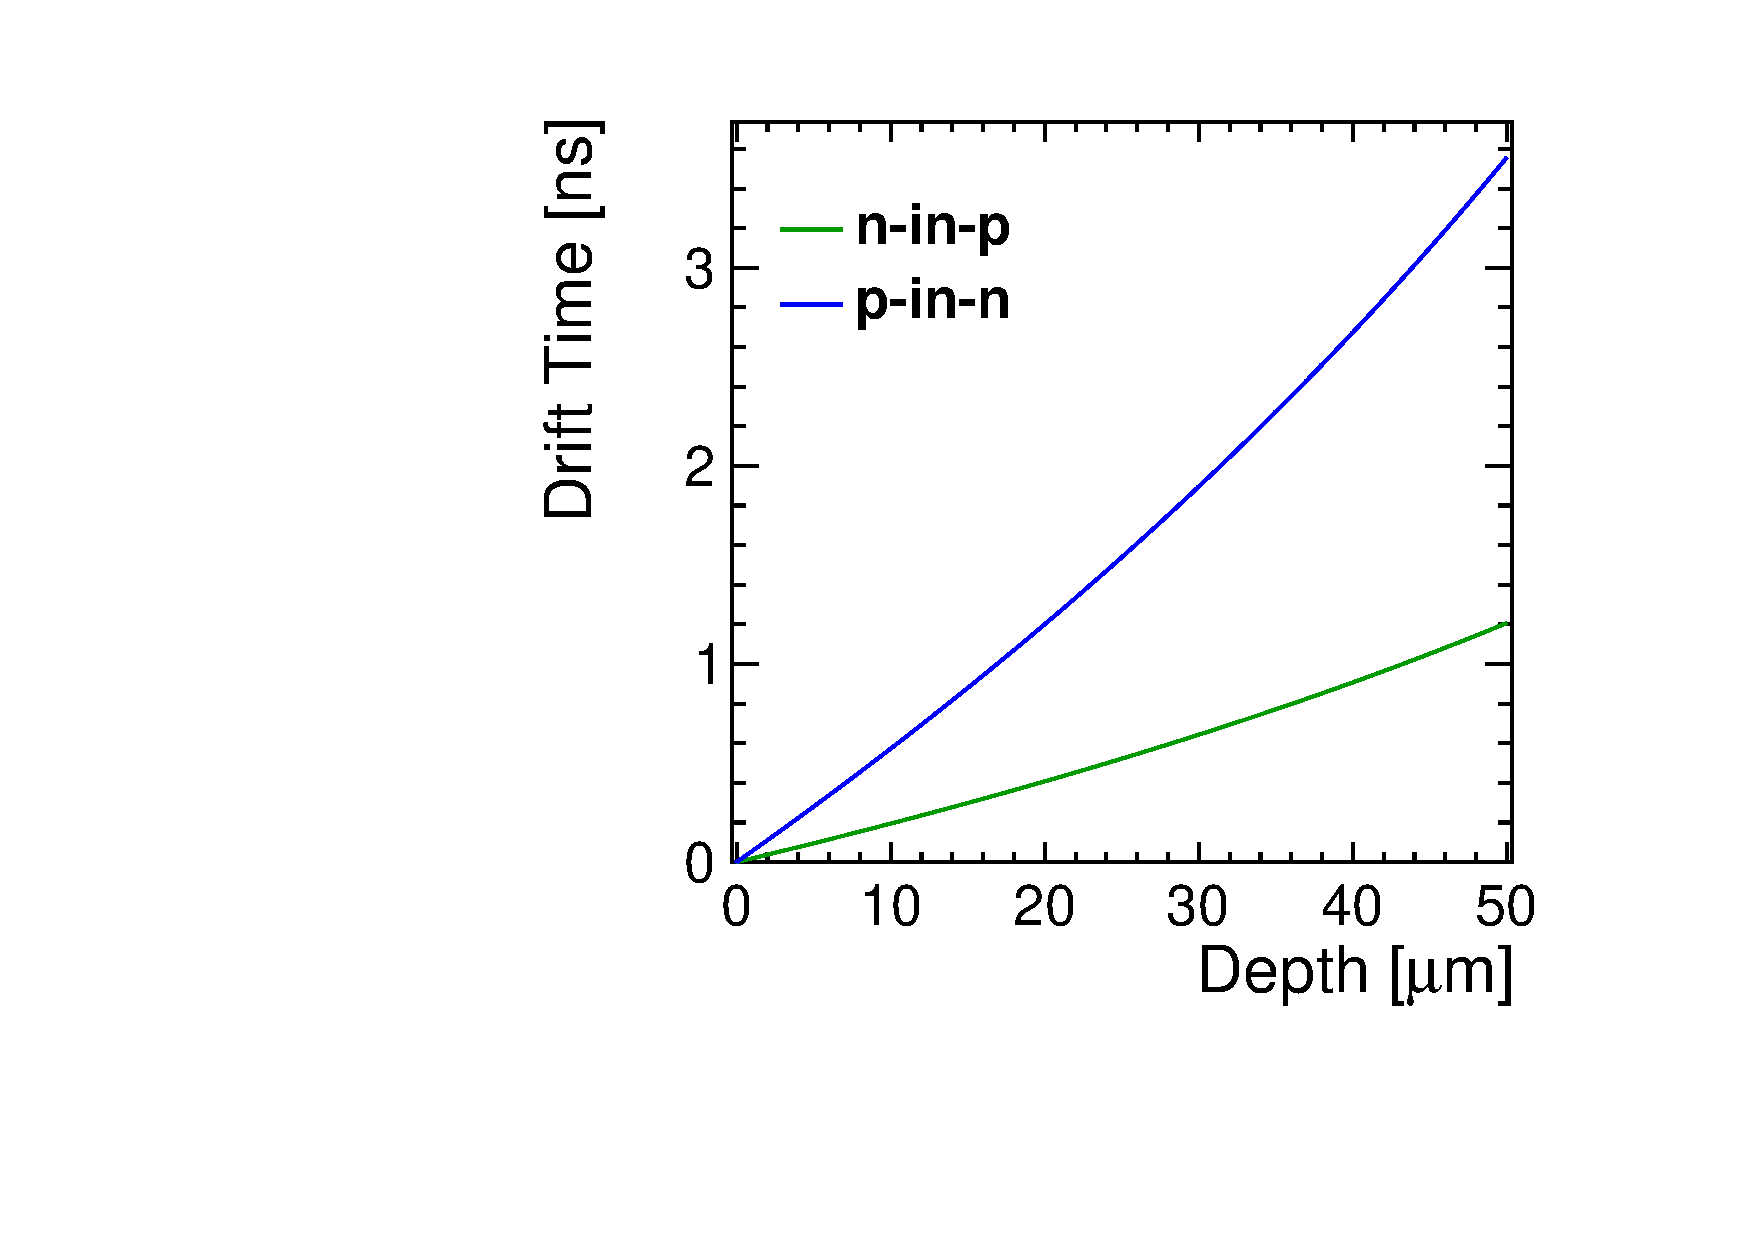
\includegraphics[width=\textwidth]{figures/ChargeSharing/DriftTime_n_vs_p_carrier.pdf}
    \caption{}\label{fig:Drift_n_vs_p}
  \end{subfigure}\hfill
  \begin{subfigure}[b]{0.45\textwidth}
    % 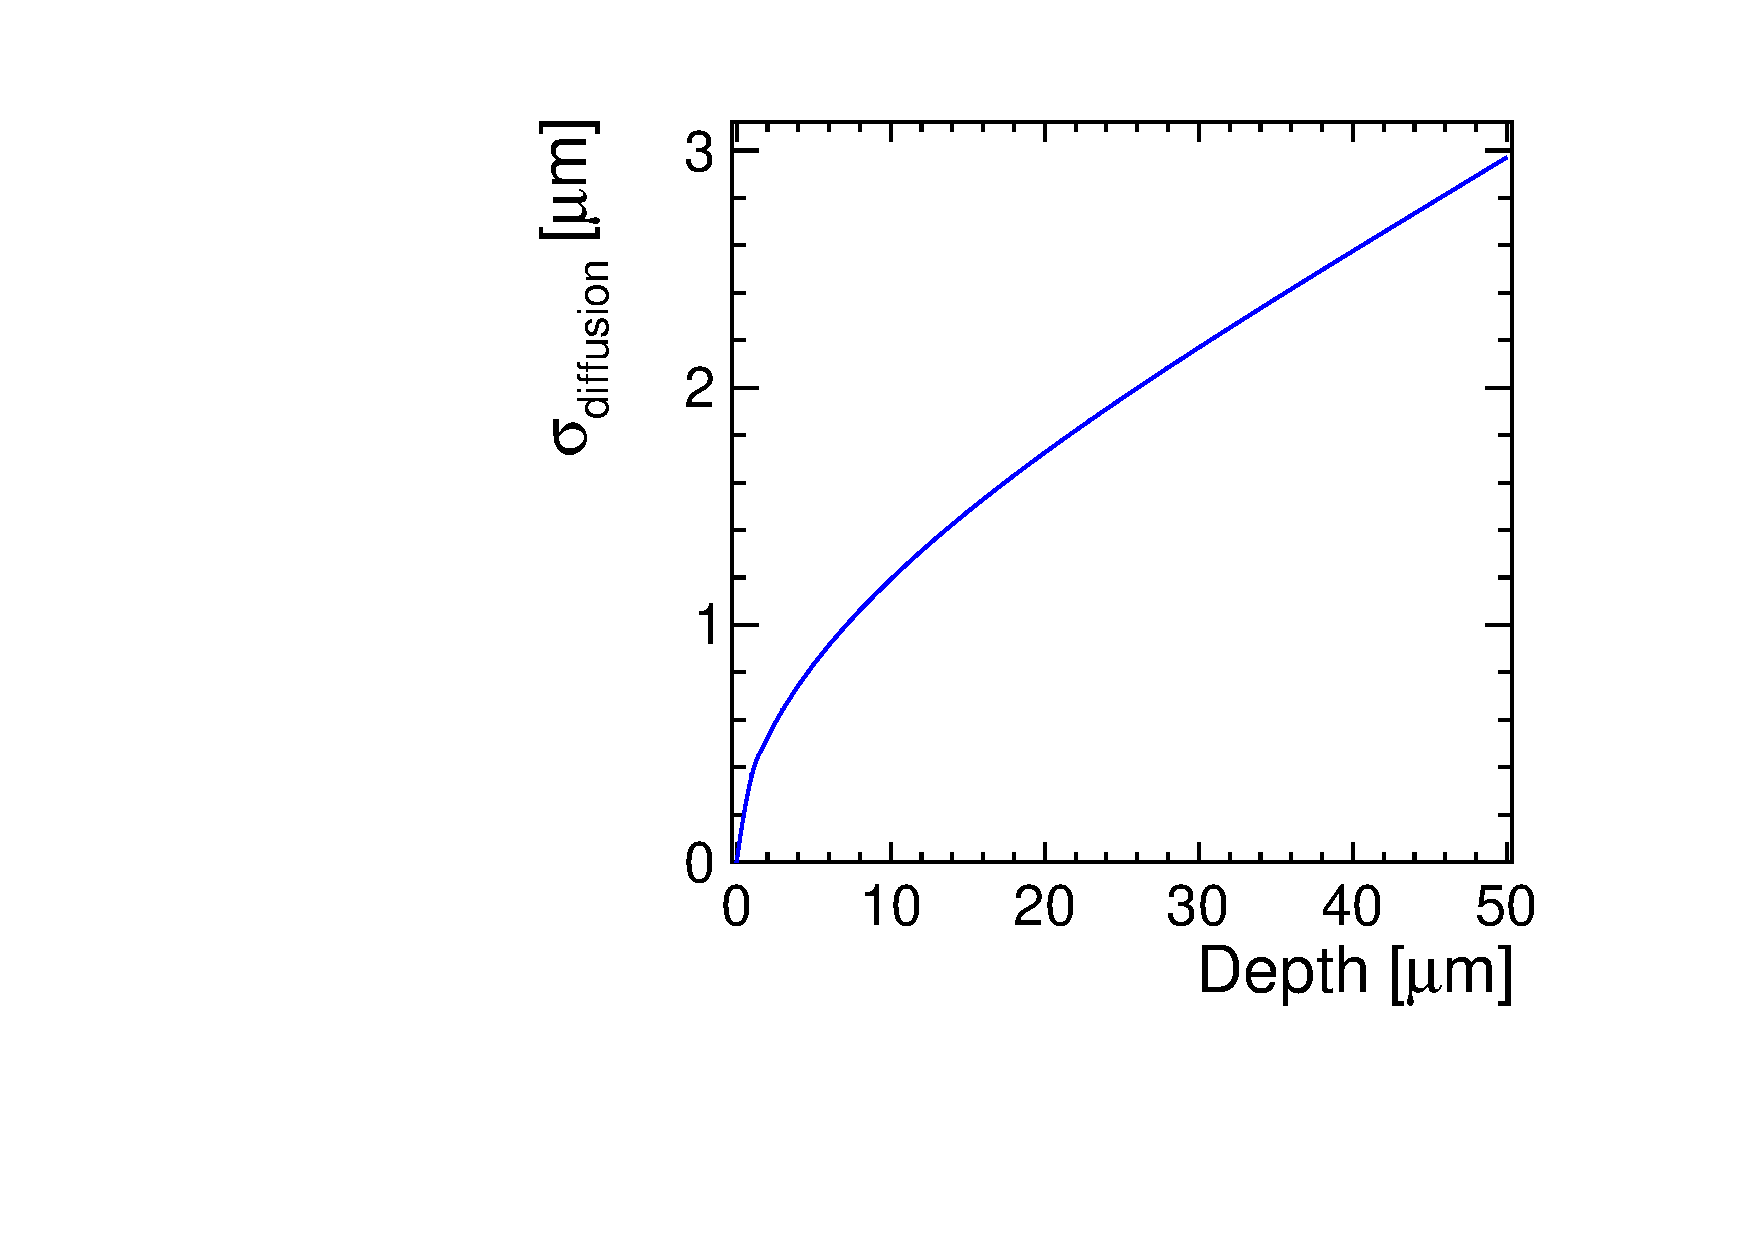
\includegraphics[width=\textwidth]{figures/ChargeSharing/Diffusion_n_vs_p_carrier.pdf}
    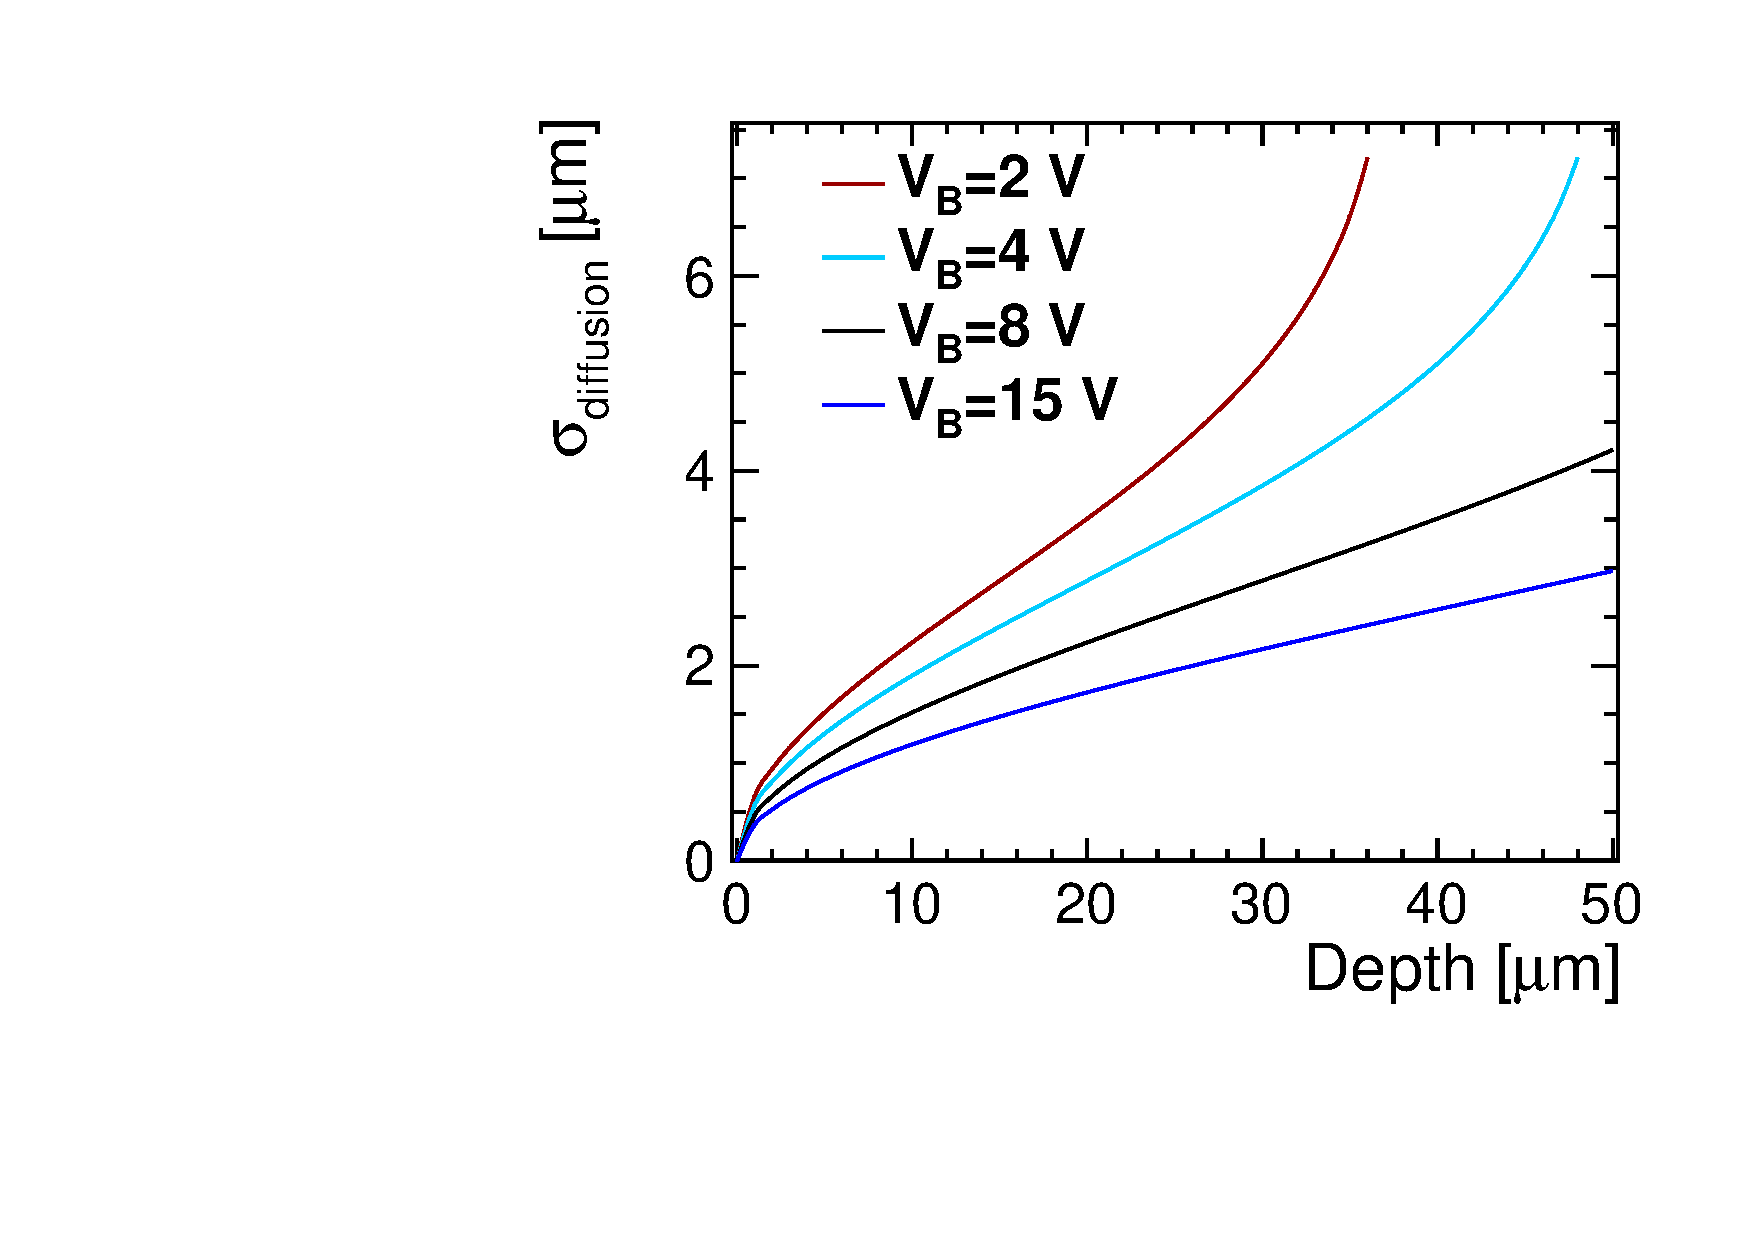
\includegraphics[width=\textwidth]{figures/ChargeSharing/Diffusion_vs_Bias.pdf}
    \caption{}\label{fig:Diffusion_n_vs_p}
  \end{subfigure}
  \caption{(a) Drift time (b) diffusion standard deviation for n and
    p-type carriers as a function of the depth in the sensor for
    different bias voltages. Diffusion does not depend on the carrier
    type. The depletion voltage is |V\textsubscript{D}|=4~V and the
    drift time is calculated considering a bias voltage of
    |V\textsubscript{B}|=15~V.}
\end{figure}

\cref{fig:Efield_n_vs_p} shows the electric field and the mobility
distribution as a function of the depth in a $50\,\micron$ thick
silicon sensor with a depletion voltage of |V\textsubscript{D}|=4~V
and biased at |V\textsubscript{B}|=15~V. The mobility in this case
stays almost constant and is not a function of the electric field
since in this case the electric field stays quite low.

\begin{figure}[htbp]
  \centering
  \begin{subfigure}[b]{0.45\textwidth}
    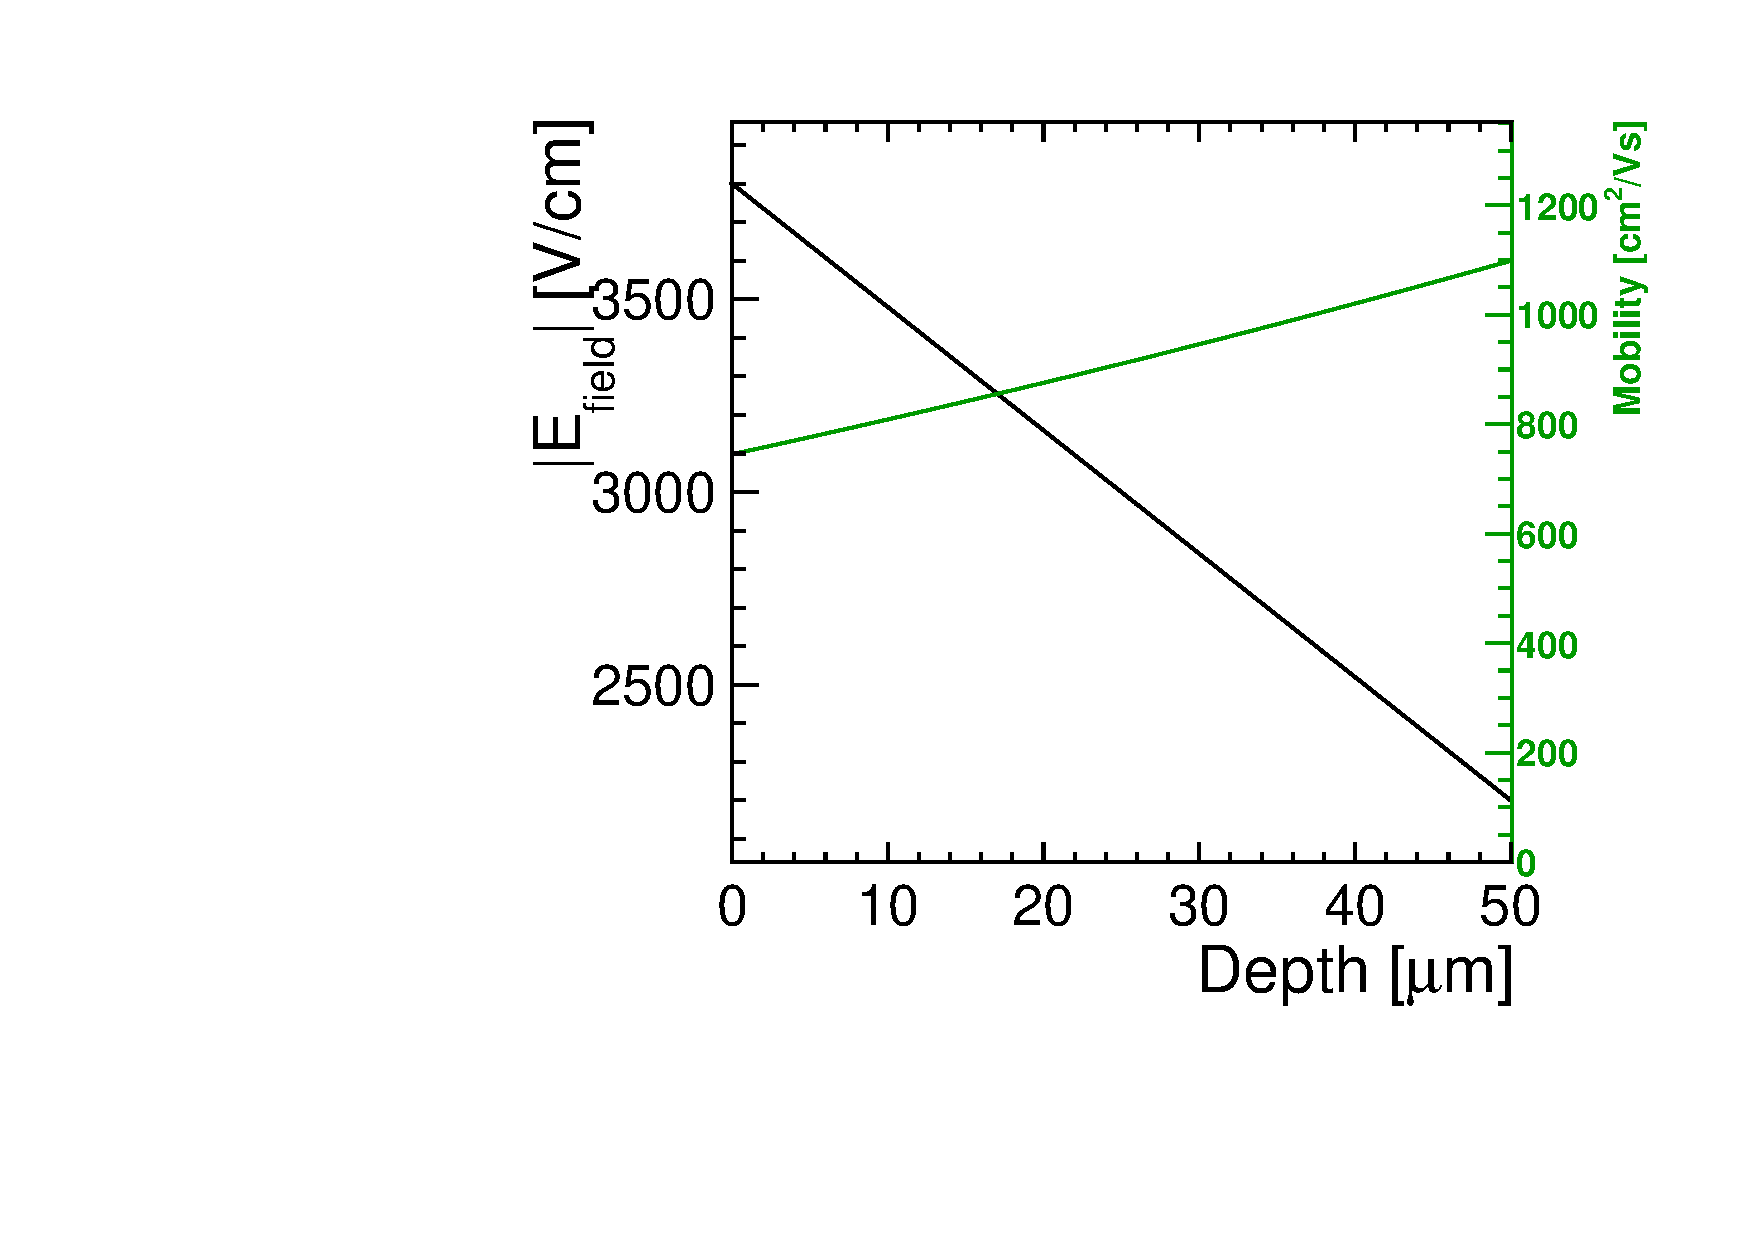
\includegraphics[width=\textwidth]{figures/ChargeSharing/Efield_mob_n_carrier.pdf}
    \caption{}
  \end{subfigure}\hfill
  \begin{subfigure}[b]{0.45\textwidth}
    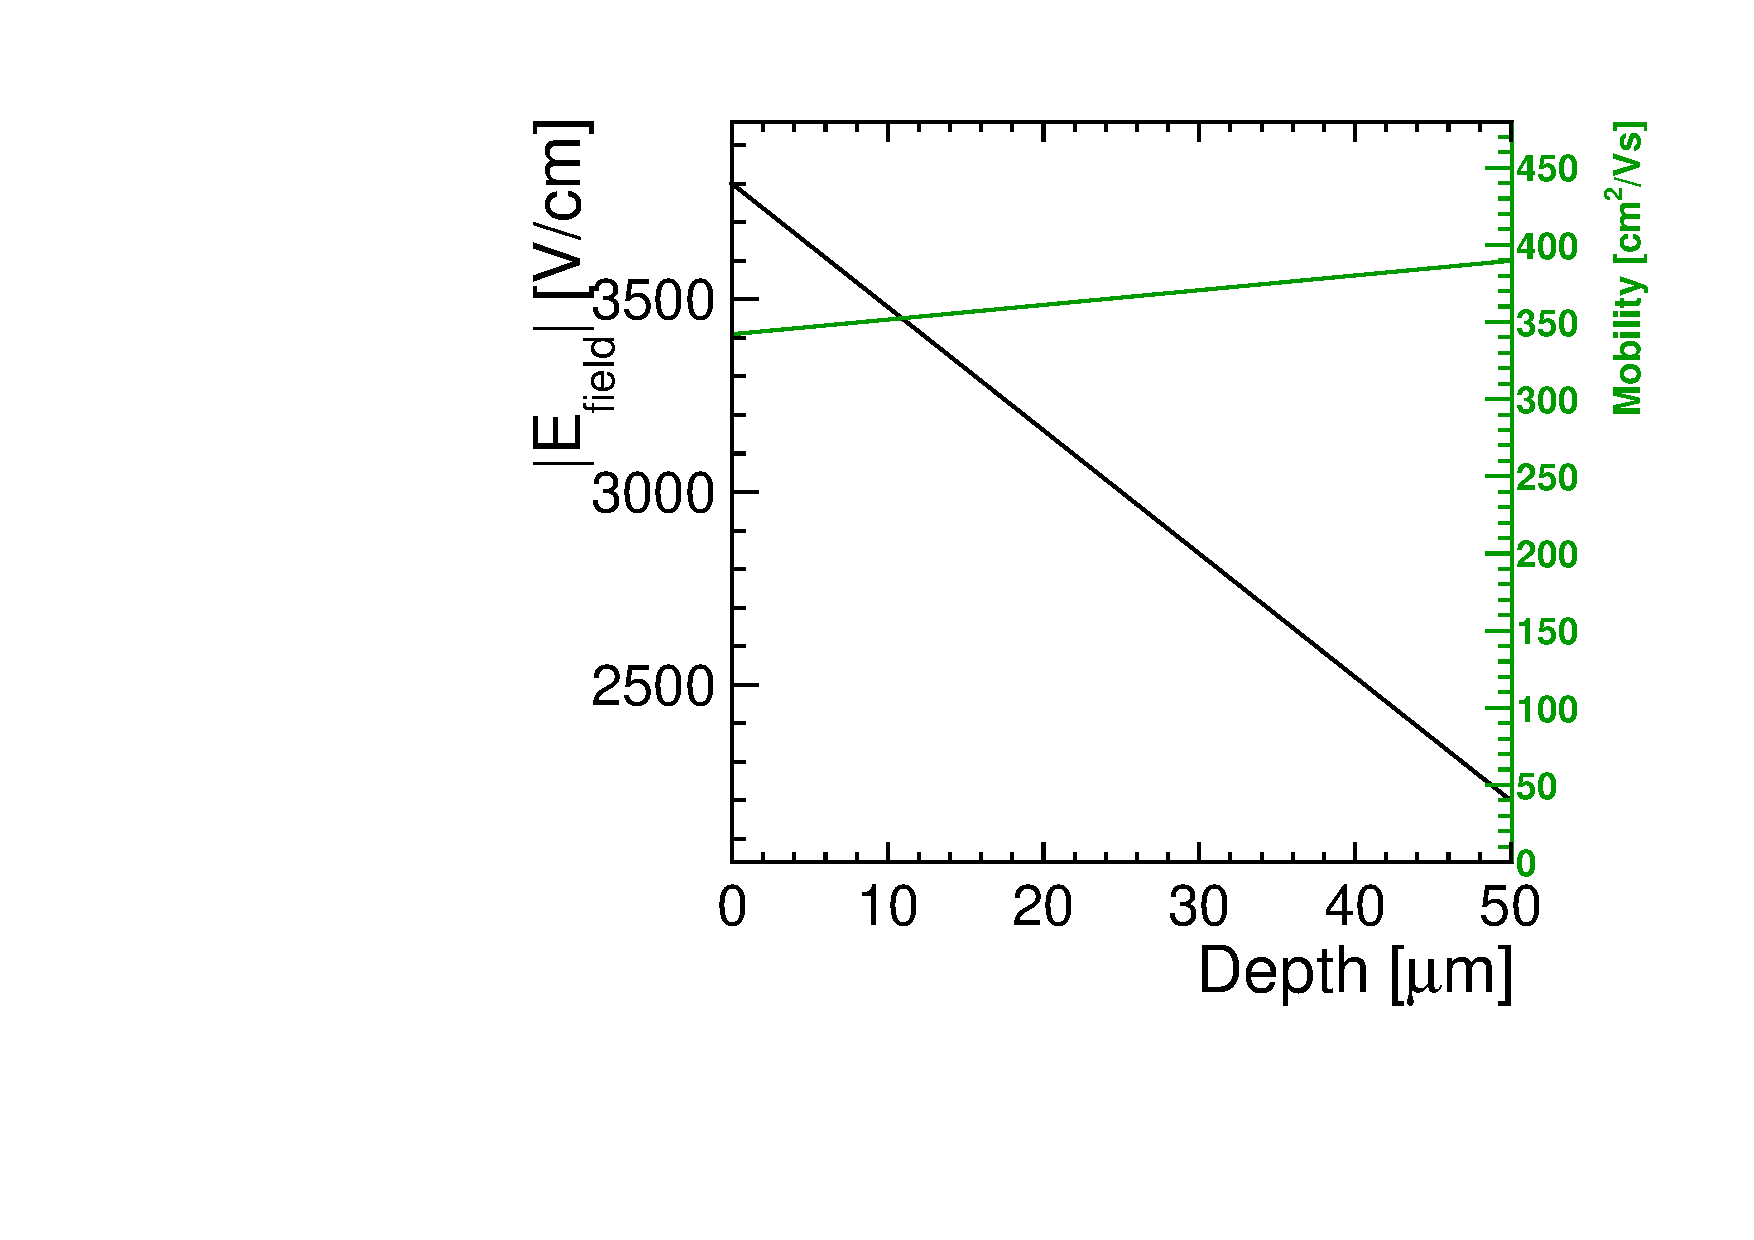
\includegraphics[width=\textwidth]{figures/ChargeSharing/Efield_mob_p_carrier.pdf}
    \caption{}
  \end{subfigure}
  \caption{The electric field and the mobility as a function of the
    depth for (a) n-type carriers and (b) p-type
    carriers.}\label{fig:Efield_n_vs_p}
\end{figure}

%% --------------------------------------------- %%
%% \subsection{TCAD simulations}

%%\newpage
\section{Pixelated silicon sensors properties}

Previously, we have reviewed the properties of a pn-junction as it is
the building block of pixel detectors. By segmenting the electrodes on
a pn-junction a pixel detector is obtained. The highly doped
electrodes, which can be n or p-type, are introduced through a mask to
form a pixel matrix with ion implantation. Each pixel forms an
independent pn-junction and the gaps between the pixels are
electrically controlled to isolate a pixel from its neighbouring
diodes. An aluminum layer deposited on the electrodes provides the
external bias voltage and signal path to the readout electronics with
a low resistance. 

This thesis focuses on hybrid pixel detectors where the electronics
for the readout and sensors are produced separately and mated using
bumps. Matrices of pixel detectors can be put together to cover larger
surfaces. \cref{fig:pixelCell} illustrates schematically the basic
building block of a hybrid pixel detector with only one pixel. An
ionising particle traversing the detector, creates charges in the
depletion region of the sensor. The charge carriers move under the
action of the applied electric field. The signal produced is acquired
by an electronics chip.

\begin{figure}[htbp]
  % \begin{wrapfigure}{r}{0.5\textwidth} 
  \centering
  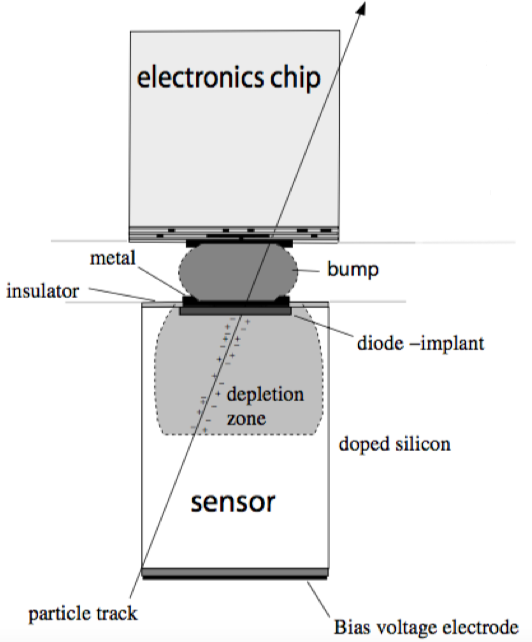
\includegraphics[width=0.5\textwidth]{figures/ChargeSharing/PixelCell.png}
  \caption{Schematic layout of one pixel cell in a hybrid pixel
    detector. From~\cite{Rossi:976471}.}
  \label{fig:pixelCell}
  % \end{wrapfigure}
\end{figure}

In the following sections, we introduce Ramo's theorem which describes
how the charge carriers are collected by the readout electrodes. Also,
an introduction to in-pixel studies done with pixel detectors is given
later when studying the spatial resolution for different readout chip
configurations.


%\subsection{Silicon sensors types}
%\subsection{Leakage current}
\subsection{Charge collection and Ramo's theorem: induced charge}
\label{sec:RamoTheorem}

Previously, we have seen that due to incident radiation, a signal is
produced by the motion of charge carriers in the detector. We can
naively interpret this statement as the signal is formed with a delay
when the charge carriers are collected by the electrodes. But in
reality, such a delay does not exist and a signal pulse is created
immediately after a charge carrier starts its motion to the
electrodes. When the last charge carriers arrive at the collecting
electrodes, the charge induction process ends and the signal pulse is
fully developed. The timing evolution of the signal is important in
understanding the timing properties of detectors. In the following, we
derive the induced charge in a pixel detector.

For the calculation of the induced charge, first, consider the simple
example of a charge $q$ near an infinitely large electrode with all
the electric field lines terminating on the electrode. The Gauss's
law, for a surface $S$ surrounding the charge is expressed as:

\begin{equation}
\oint_{s} \vec{E} \cdot d\vec{a}=q\; .
\label{eq:GaussLaw}
\end{equation}

The induced charge obtained by integrating over a Gaussian surface
enclosing only the electrode is $-q$. Now, let's consider two parallel
electrodes with a charge $q$ in between as showin in
\cref{fig:InducedCharge_parallelPlates}. If the charge is placed
midway between the two parallel plates, it induces equal charge of
$-q/2$ on the both electrodes as half of the electric field lines end
up on the higher and the other half on the lower electrode. When the
charge moves closer to a plate rather than the other, the induced
charge will be higher for the closer plate.

The induced charge can not be observed directly but its change can be
measured when the two electrodes are connected in a closed circuit
(like a pixel detector) as it produces an induced current.

\begin{figure}[htbp]
  \centering
  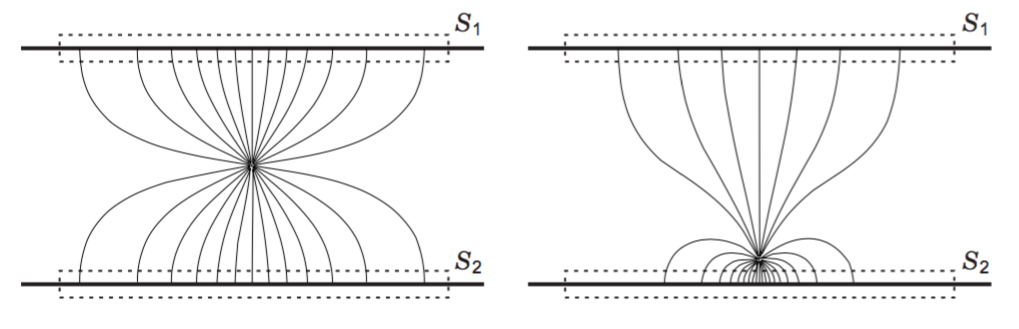
\includegraphics[width=0.8\textwidth]{figures/Ramo/InducedCharge_parallelPlates.png}
  \caption{The charge induced on two parallel plates depending on the
    position of the charge $q$. From~\cite{Spieler2005}.}
  \label{fig:InducedCharge_parallelPlates}
\end{figure}

Ramo's theorem~\cite{Ramo:1939vr} describes the time evolution of the
induced current created in a detector. The induced current on the
electrodes is described as a function of the weighting potential
$\Phi$ which describes the coupling of a charge to an electrode. The
weighting potential is defined for a specific electrode. In Ramo's
theorem, it is obtained by setting the potential of the electrode to 1
and setting all other electrodes to potential 0. \cref{eq:RamoCharge}
describes the induced charge $Q_k$ on electrode $k$ if a charge q
moves along any path from position $z_0$ to $z_p$:
\begin{equation}
    Q_{k}=q \cdot [\Phi_k(z_p)-\Phi_k(z_0)] \; .
   \label{eq:RamoCharge} 
  \end{equation}

  It is important to note that the weighting potential (field) is
  different from the electric potential (field). The electric field
  determines the drift trajectory and velocity of the charge carriers
  whereas the weighting field depends only on the geometry of the
  electrodes and defines how the charge motion induces a charge to a
  specific electrode. In the specific case of two-electrode
  configuration the electric and the weighting fields are the same.


  \cref{fig:RamoTCAD} shows the weighting field and potential
  distributions calculated using TCAD simulations~\cite{synopsysTCAD}
  (c.f. \cref{sec:TCAD}). For this study, we consider a silicon sensor
  with 5 pixels (marked out with dashed lines), having a thickness of
  200~\micron and over-depleted with a bias voltage of \SI{50}{\volt}
  on the back-side. First, \SI{0}{\volt} is applied to all the
  electrodes and then \SI{1}{\volt} is applied to the
  electrode~$k$. By taking the difference between the two
  configurations, the weighting potential and field are obtained.


\begin{figure}[htbp]
  \centering
  \begin{subfigure}[b]{0.45\textwidth}
    \centering
    \begin{tikzpicture}
      \node[anchor=south west,inner sep=0] (image) at (0,0){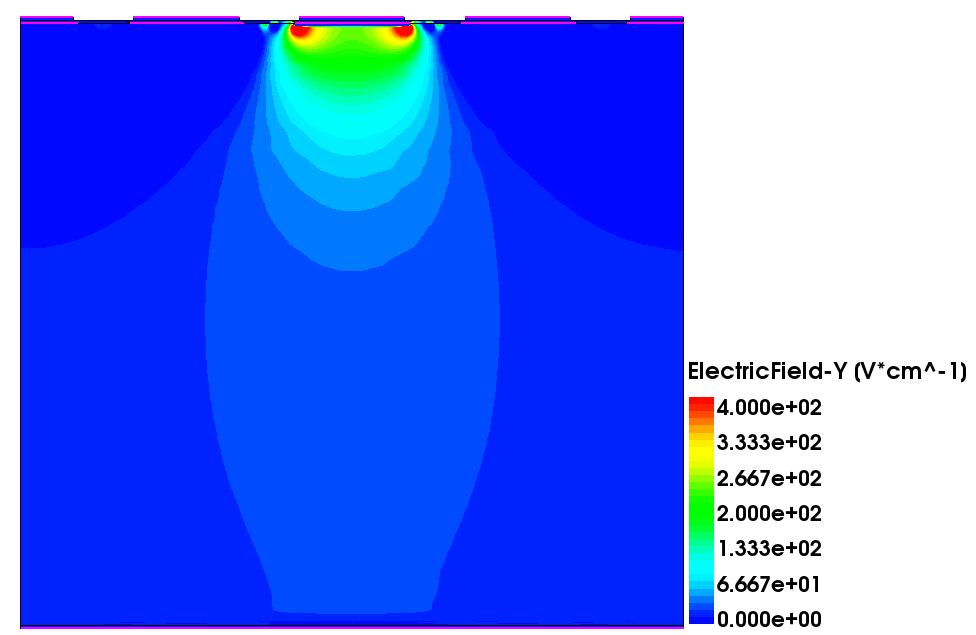
\includegraphics[width=\textwidth]{figures/Ramo/EfieldY_Ramo.png}};
      \begin{scope}[x={(image.south east)},y={(image.north west)}]
        \node[above, color=black] at (0.35, 1) {electrode $k$};

        \draw[->, thick] (0, 1)--(0, -0.1) node[below]{Depth
          $z$~$[\micron]$};
        \draw[-] (-0.01, 0.01) -- (0.01, 0.01) node[left] {200};
        \draw[-] (-0.01, 0.97) -- (0.01, 0.97) node[left] {0};

        \draw[-, dashed] (0.11, 0.95)--(0.11, 0.02);
        \draw[-, dashed] (0.27, 0.95)--(0.27, 0.02);
        \draw[-, dashed] (0.45, 0.95)--(0.45, 0.02);
        \draw[-, dashed] (0.62, 0.95)--(0. 62, 0.02);

        % \draw[help lines,xstep=.1,ystep=.1] (0, 0) grid (1,1);
        % \foreach \x in {0,1,...,9} { \node [anchor=north] at (\x/10,0) {0.\x}; }
        % \foreach \y in {0,1,...,9} { \node [anchor=east] at (0,\y/10) {0.\y}; }

      \end{scope}
    \end{tikzpicture} 
    \caption{Weighting field}\label{fig:WeightingFieldRamo}
  \end{subfigure}\hfill
  \begin{subfigure}[b]{0.45\textwidth}
    \centering
    \begin{tikzpicture}
      \node[anchor=south west,inner sep=0] (image) at (0,0){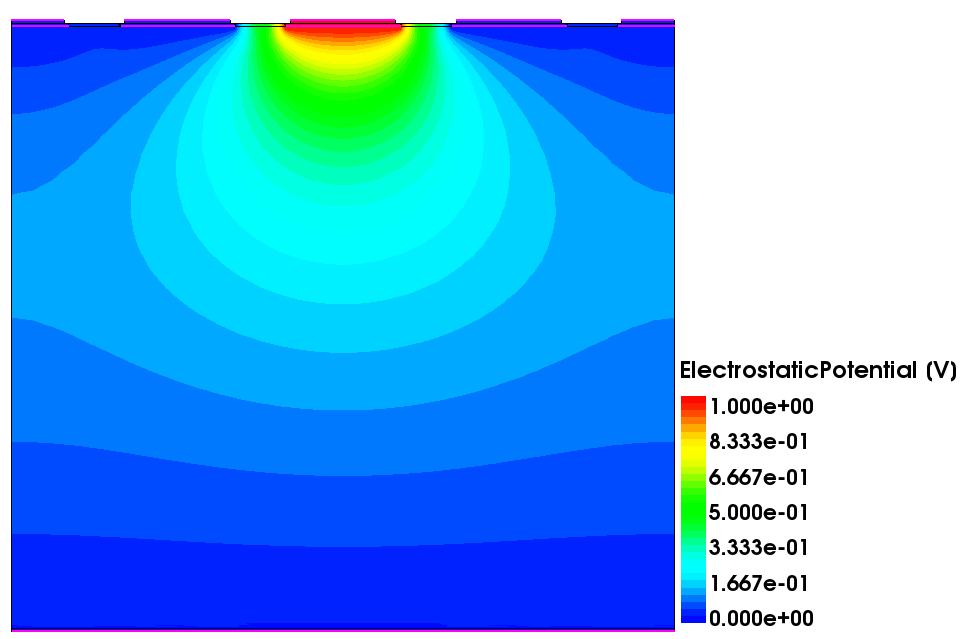
\includegraphics[width=\textwidth]{figures/Ramo/RamoPotential.png}};
      \begin{scope}[x={(image.south east)},y={(image.north west)}]
        \node[above, color=black] at (0.35, 1) {electrode $k$};

        \draw[->, thick] (0, 1)--(0, -0.1) node[below]{Depth
          $z$~$[\micron]$};
        \draw[-] (-0.01, 0.01) -- (0.01, 0.01) node[left] {200};
        \draw[-] (-0.01, 0.97) -- (0.01, 0.97) node[left] {0};

        \draw[-, dashed] (0.11, 0.95)--(0.11, 0.02);
        \draw[-, dashed] (0.27, 0.95)--(0.27, 0.02);
        \draw[-, dashed] (0.45, 0.95)--(0.45, 0.02);
        \draw[-, dashed] (0.62, 0.95)--(0. 62, 0.02);

      \end{scope}
    \end{tikzpicture} 
    \caption{Weighting potential}\label{fig:WeightingPotentialRamo}
  \end{subfigure} 
  \caption{The weighting field and potential on electrode $k$.}\label{fig:RamoTCAD}
\end{figure}

The weighting potential for different hit positions on the x-axis is
shown in \cref{fig:RamoTCADCuts}. Since, the total charge collected by
the electrode $k$ depends only on the depth positions $z_0$ and $z_p$,
in the absence of the radiation-induced damages (which would affect
the distributions of the electric and weighting fields), the Ramo
theorem can be neglected. The charge carriers drift following the
electric field distribution and the diffusion causes multi-pixel hits.

\begin{figure}[htbp]
  \centering
  \begin{subfigure}[b]{0.48\textwidth}
    \centering
    \begin{tikzpicture}
      \node[anchor=south west,inner sep=0] (image) at
      (0,0){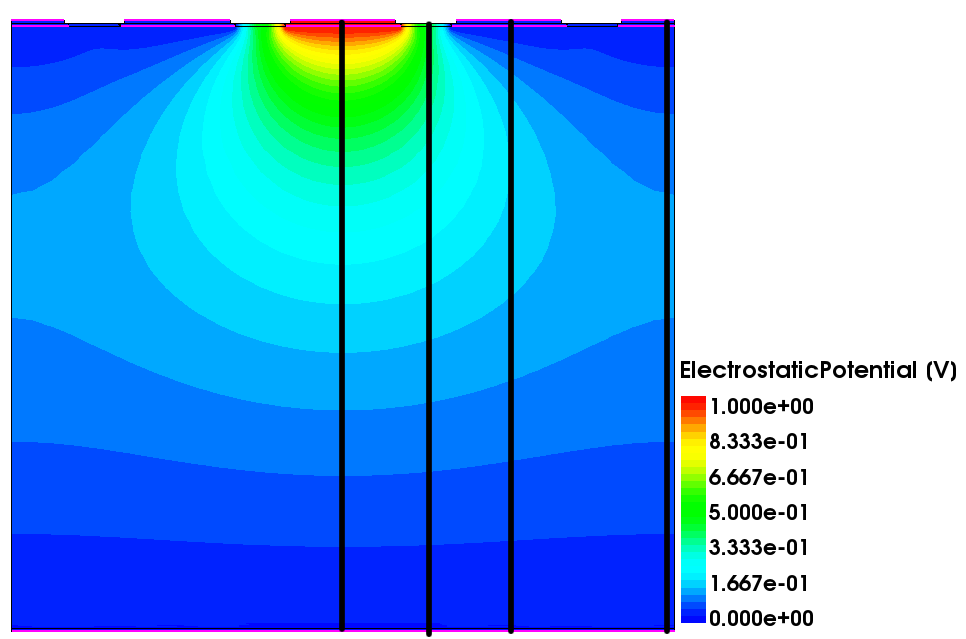
\includegraphics[width=\textwidth]{figures/Ramo/RamoPotential_cuts.png}};
      \begin{scope}[x={(image.south east)},y={(image.north west)}]
        \draw[->, thick] (-0.1, 1)--(0.73, 1) node[right]{$x$~$[\micron]$};
        \draw[->, thick] (0, 1.1)--(0, -0.1) node[below]{Depth $z$~$[\micron]$};
        \draw[-] (0.355, 1.01) -- (0.355, 0.99) node[above] {0};
        \draw[-] (0.445, 1.01) -- (0.445, 0.99) node[above] {27.5};
        \draw[-] (0.533, 1.01) -- (0.533, 0.99) node[above] {55};
        \draw[-] (0.69, 1.01) -- (0.69, 0.99) node[above] {109};


        \draw[-] (-0.01, 0.01) -- (0.01, 0.01) node[left] {200};
        \draw[-] (-0.01, 0.97) -- (0.01, 0.97) node[left] {0};
        %% \draw[help lines,xstep=.1,ystep=.1] (0, 0) grid (1,1);
        %% \foreach \x in {0,1,...,9} { \node [anchor=north] at (\x/10,0) {0.\x}; }
        %% \foreach \y in {0,1,...,9} { \node [anchor=east] at (0,\y/10) {0.\y}; }

      \end{scope}
    \end{tikzpicture} 
    \caption{}\label{fig:RamoPotentialCuts}
  \end{subfigure}\hfill
  \begin{subfigure}[b]{0.49\textwidth}
    \centering
    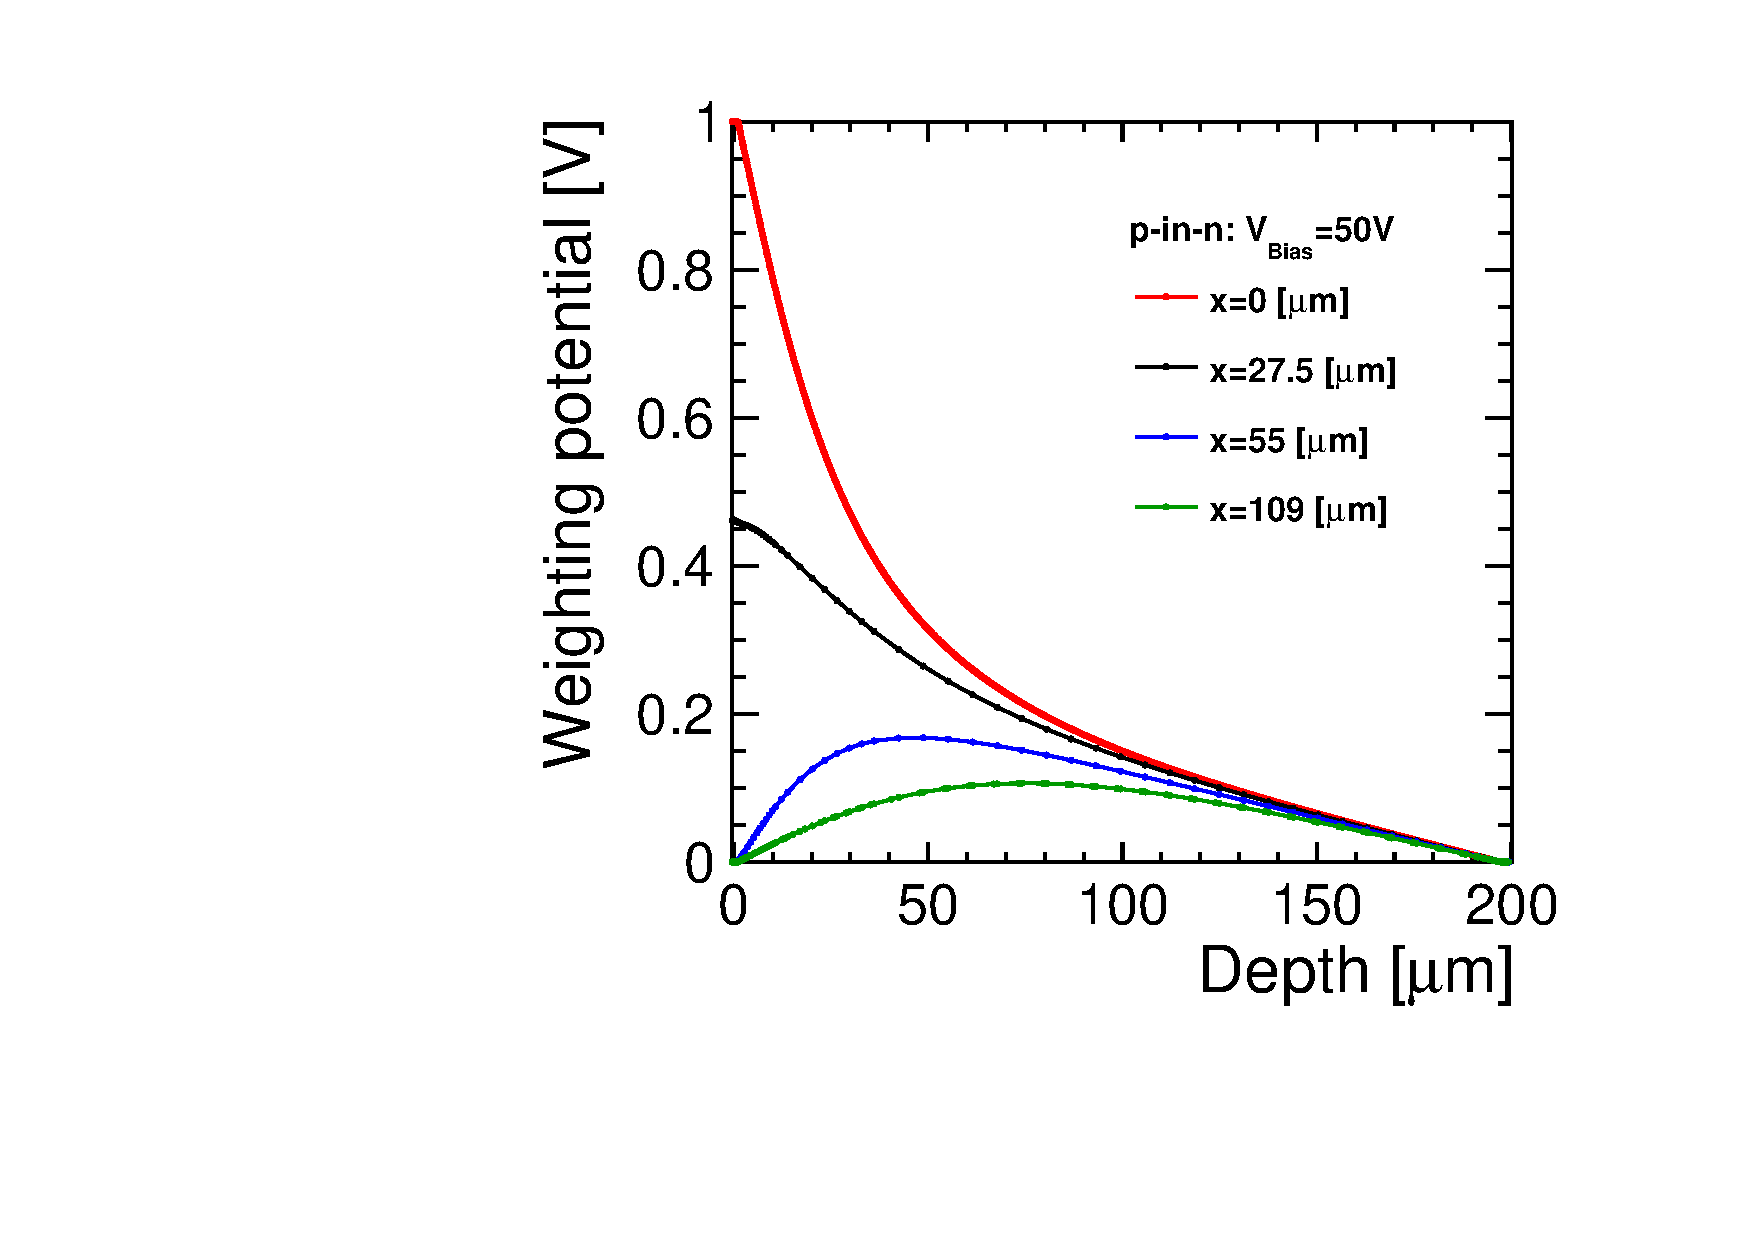
\includegraphics[width=0.9\textwidth]{figures/Ramo/WeightingPotential_1D.pdf}
    \caption{}\label{fig:RamoPotentialCuts1D}
  \end{subfigure} 
  \caption{The weighting potential for different positions on the x-axis using TCAD simulations. The detector has a thickness of $200\,\micron$.}
  \label{fig:RamoTCADCuts}
\end{figure}


\subsection{Spatial resolution}

The spatial resolution of a pixel detector is mainly determined by the
pixel pitch. But this can be improved by the readout choice (binary or
analogue), the threshold value, the charge sharing, thickness of the
detector and the reconstruction algorithm. The effect of the readout
is studied in the sections here-below.

The spatial resolution is defined by:
\begin{equation}
\sigma_{position}^2={{\int_{-p/2}^{p/2} \left(x_r-x_m\right)^2
    D\left(x_r\right) dx_r } \over { \int_{-p/2}^{p/2}
    D\left(x_r\right) dx_r }}\; ,
\label{eq:spatialRes}
\end{equation}

where $\sigma_{position}$ is the average distance between the real
impact position $x_r$ and the measured position $x_m$ of the particle
in a pixel. $D\left(x\right)$ is the hit probability density function
in a pixel. $p$ represents the pixel pitch size.

In the coming sections, the spatial resolution defined by
\cref{eq:spatialRes} is studied for different scenarios and
assumptions.

%% \begin{figure}[htbp]
%%   \centering
%%   \begin{subfigure}[b]{0.3\textwidth}
%%     \centering
%%     \begin{tikzpicture}
%%       \draw[->, thick] (-2,0)--(2,0) node[right]{$x$};
%%       \draw[->, thick] (0, -0.5)--(0, 2) node[above]{$D\left(x\right)$};
      
%%       \draw[-] (-1.5, 1) -- (-1.5, 0) node[below]{${-p \over 2}$};
%%       \draw[-] (-1.5, 1) -- (1.5, 1);
%%       \draw[-] (1.5, 1) -- (1.5, 0) node[below]{${p \over 2}$};
%%       \node[] at (0.2, 1.2) {1};
%%     \end{tikzpicture}
%%     \caption{}\label{fig:SpatResBinary}
%%   \end{subfigure}\hfill
%%   \begin{subfigure}[b]{0.3\textwidth}
%%     \centering
%%     \begin{tikzpicture}
%%       \draw[->, thick] (-2,0)--(2,0) node[right]{$x$};
%%       \draw[->, thick] (0, -0.5)--(0, 2) node[above]{$D\left(x\right)$};
      
%%       \draw[-] (-0.7, 1) -- (-0.7, 0) node[below]{\tiny ${{-(p-s)}\over 2}$};
%%       \draw[-] (-0.7, 1) -- (0.7, 1);
%%       \draw[-] (0.7, 1) -- (0.7, 0) node[below]{\tiny ${(p-s)\over 2}$};
%%       \node[] at (0.2, 1.2) {1};
%%       \draw[-] (-1.5, 0.1) -- (-1.5, 0) node[below] {${-p \over 2}$};
%%       \draw[-] (1.5, 0.1) -- (1.5, 0) node[below] {${p \over 2}$};
%%     \end{tikzpicture}
%%     \caption{}\label{fig:SpatResBinaryChargeSharing}
%%   \end{subfigure}\hfill
%%   \begin{subfigure}[b]{0.3\textwidth}
%%     \centering
%%     \begin{tikzpicture}
%%       \draw[->, thick] (-2,0)--(2,0) node[right]{$x$};
%%       \draw[->, thick] (0, -0.5)--(0, 2) node[above]{$D\left(x\right)$};
      
%%       \draw (-1.5,0) to[out=0, in=-120] (-0.9,0.2) to[out=60, in=180](-0.3, 1)--(0,1);
%%       \draw (0,1)--(0.3, 1) to [out=-20, in=120] (0.9,0.2) to[out=-60,
%%       in=0] (1.5,0);

%%       \draw[-] (-1.5, 0.1) -- (-1.5, 0) node[below] {${-p \over 2}$};
%%       \draw[-] (1.5, 0.1) -- (1.5, 0) node[below] {${p \over 2}$};

%%       \draw[-] (-0.5, 0.1) -- (-0.5, 0) node[below] {\tiny ${-(p-s) \over 2}$};
%%       \draw[-] (0.5, 0.1) -- (0.5, 0) node[below] {\tiny ${(p-s) \over 2}$};

%%       \node[] at (0.2, 1.2) {1};
%%     \end{tikzpicture}
%%     \caption{}\label{fig:SpatResAnaglogChargeSharing}
%%   \end{subfigure}
%%   \caption{(a) Binary readout. (b) Binary readout with charge
%%     sharing. (c) Analog readout with charge sharing.}\label{fig:SpatialResolution}
%% \end{figure}



\subsubsection{Binary readout} \label{sec:binaryReadout}
The simplest case for the resolution computation is to consider a
binary readout with single threshold for signal and noise
discrimination. For a pixel centered at 0 and having a pitch $p$ with
a probability density function as illustrated in
\cref{fig:SpatResBinary}, the following assumptions are considered:

\begin{itemize}
\item The threshold is adjusted in a way to fire one pixel per
  particle track.
\item Only hit positions between $-p/2$ and $p/2$ trigger a signal in
  pixel 0.
\item A uniform density of particles hit the detector ($D\left(x\right)=1$).
\end{itemize}


The average difference between the real position ($x_r$) and the
measured position ($x_m=0$) of the particle in a pixel is calculated
using \cref{eq:spatialRes} \cite{Rossi:976471}:
\begin{equation}
\sigma_{position}^2={{\int_{-p/2}^{p/2} \left(x_r\right)^2
    1 dx_r } \over { \int_{-p/2}^{p/2}
    1 dx_r }}={p^2 \over 12} \; ,
\label{eq:spatialResBinary}
\end{equation}
which results in a spatial resolution of:
\begin{equation}
\sigma_{position}={p \over \sqrt{12}} \;.
\label{eq:sigmaposBinary}
\end{equation}

\begin{figure}[htbp]
  \centering
  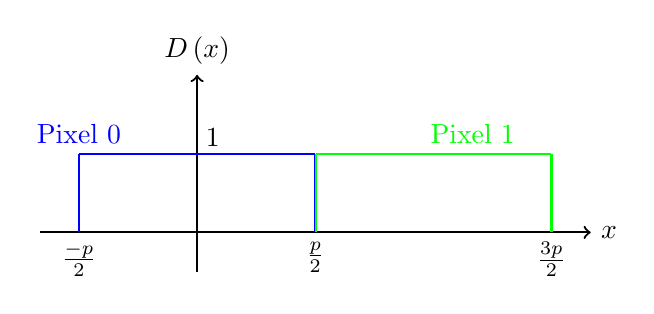
\begin{tikzpicture}
    \begin{scope}
      \draw[->, thick] (-2,0)--(5,0) node[right]{$x$};
      \draw[->, thick] (0, -0.5)--(0, 2) node[above]{$D\left(x\right)$};
      
      \draw[-, blue, thick] (-1.5, 1) -- (-1.5, 0);
      \node[below] at (-1.5, 0) {${-p \over 2}$};
      \draw[-, blue, thick] (-1.5, 1) -- (1.5, 1);
      \draw[-, blue, thick] (1.5, 1) -- (1.5, 0);
      \node[below] at (1.5, 0) {${p \over 2}$};
      \node[] at (0.2, 1.2) {1};
      \node[above, blue] at (-1.5, 1) {Pixel 0};

      \draw[-, green, thick] (1.51, 1) -- (1.51, 0);
      \draw[-, green, thick] (1.51, 1) -- (4.5, 1);
      \draw[-, green, thick] (4.5, 1) -- (4.5, 0);
      \node[below] at (4.5, 0) {${{3p} \over 2}$};
      \node[above, green] at (3.5, 1) {Pixel 1};
    \end{scope}
  \end{tikzpicture}
  \caption{The hit probability density function for two neighbouring
    pixels (pixel 0 and pixel 1) when a binary readout is used to
    acquire the sensor pulse.}
  \label{fig:SpatResBinary}
\end{figure}

This simple model shows the worst resolution achieved and is only
dependent on the pitch size (geometry of the pixels). In reality, with
charge sharing, the signal of a particle track is shared between
several pixels and depending on the readout threshold more than one
pixel can be fired which is called a \textit{cluster} of pixels. The
resolution is therefore improved as described in
\cref{sec:resolutionBinarySharing,sec:resolutionAnalogSharing}.

\subsubsection{Binary readout and charge sharing}
\label{sec:resolutionBinarySharing}

The threshold of the readout electronics is usually set as low as
possible which can result in more than one pixel hit per particle
track. In this case, the charge is shared between two or more pixels
(called a cluster). Multi-hit clusters improve the resolution of
\cref{eq:sigmaposBinary}. \cref{fig:SpatResBinaryChargeSharing}
illustrates the charge sharing between two pixels. If a track passes
close to the edge of a pixel (within a distance of $s\over 2$ close to
the edge), then the neighbouring pixel is also fired. For events
triggering single-hit events, the spatial resolution in pixel 0 for
1-hit clusters is given by:

\begin{equation}
\sigma_{position}^2={{\int_{-(p/2-s/2)}^{(p/2-s/2)} \left(x_r\right)^2
    1 dx_r } \over { \int_{-(p/2-s/2)}^{(p/2-s/2)}
    1 dx_r }}={(p-s)^2 \over 12} \; .
\label{eq:spatialResCharge sharing_1hit}
\end{equation}

For two-hit clusters, the spatial resolution is given by:
\begin{equation}
\sigma_{position}={s \over \sqrt{12}} \; .
\label{eq:spatialResChargeSharing_2hit}
\end{equation}



\begin{figure}[htbp]
  \centering
  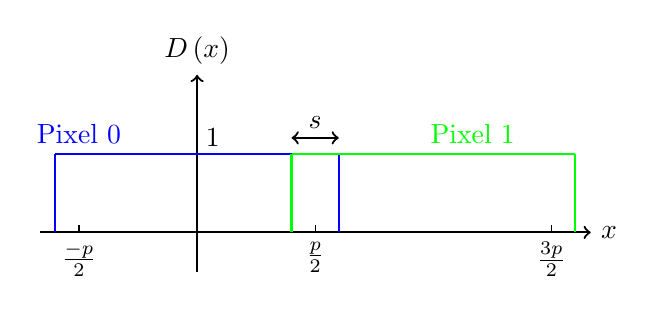
\begin{tikzpicture}
    \begin{scope}
      
      \draw[->, thick] (-2,0)--(5,0) node[right]{$x$};
      \draw[->, thick] (0, -0.5)--(0, 2) node[above]{$D\left(x\right)$};
      
      \draw[-, blue, thick] (-1.8, 1) -- (-1.8, 0);

      \draw[-] (-1.5, 0) -- (-1.5, 0.1);
      \node[below] at (-1.5, 0) {${-p \over 2}$};
      \draw[-, blue, thick] (-1.8, 1) -- (1.8, 1);
      \draw[-, blue, thick] (1.8, 1) -- (1.8, 0);

      \draw[-] (1.5, 0) -- (1.5, 0.1);
      \node[below] at (1.5, 0) {${p \over 2}$};
      \node[] at (0.2, 1.2) {1};
      \node[above, blue] at (-1.5, 1) {Pixel 0};
      
      \draw[-, green, thick] (1.2, 1) -- (1.2, 0);
      \draw[-, green, thick] (1.2, 1) -- (4.8, 1);
      \draw[-, green, thick] (4.8, 1) -- (4.8, 0);
      \draw[-] (4.5, 0) -- (4.5, 0.1);
      \node[below] at (4.5, 0) {${{3p} \over 2}$};
      \node[above, green] at (3.5, 1) {Pixel 1};

      \draw[<->, thick] (1.2, 1.2)--(1.8, 1.2);
      \node[above] at (1.5, 1.2) {$s$};
      
    \end{scope}
  \end{tikzpicture}
  \caption{The hit probability density function for two neighbouring
    pixels (pixel 0 and pixel 1) considering charge sharing between
    the two pixels when a binary readout is used to acquire the sensor
    pulse. For a track passing in the edge of the two pixels, within a
    distance of $s$/2 close to the edge, pixel 0 and pixel 1 are
    fired.}\label{fig:SpatResBinaryChargeSharing}
  % Binary readout with charge sharing.
\end{figure}

The average resolution considering single and multi-hit clusters is
given by:
\begin{equation}
{\sigma_{Total}^{2}}={{\left(p-s\right)^{2}} \over 12}+{{s^2}\over12} \; .
\label{eq:spatialResChargeSharingTotal}
\end{equation}

The optimal average spatial resolution is obtained for $s=p/2$ as
shown in \cref{fig:sigmaTotal} for three pixel pitches of
$p=15\,\micron$, $p=25\,\micron$ and $p=55\,\micron$. This means that
the number of single-hit and multi-hit clusters is the same. But, in
this situation one is not able to distinguish between one track
triggering two pixels and two tracks hitting the sensor within $2p$.

\begin{figure}[htbp] \centering
  \begin{subfigure}[b]{0.3\textwidth}
    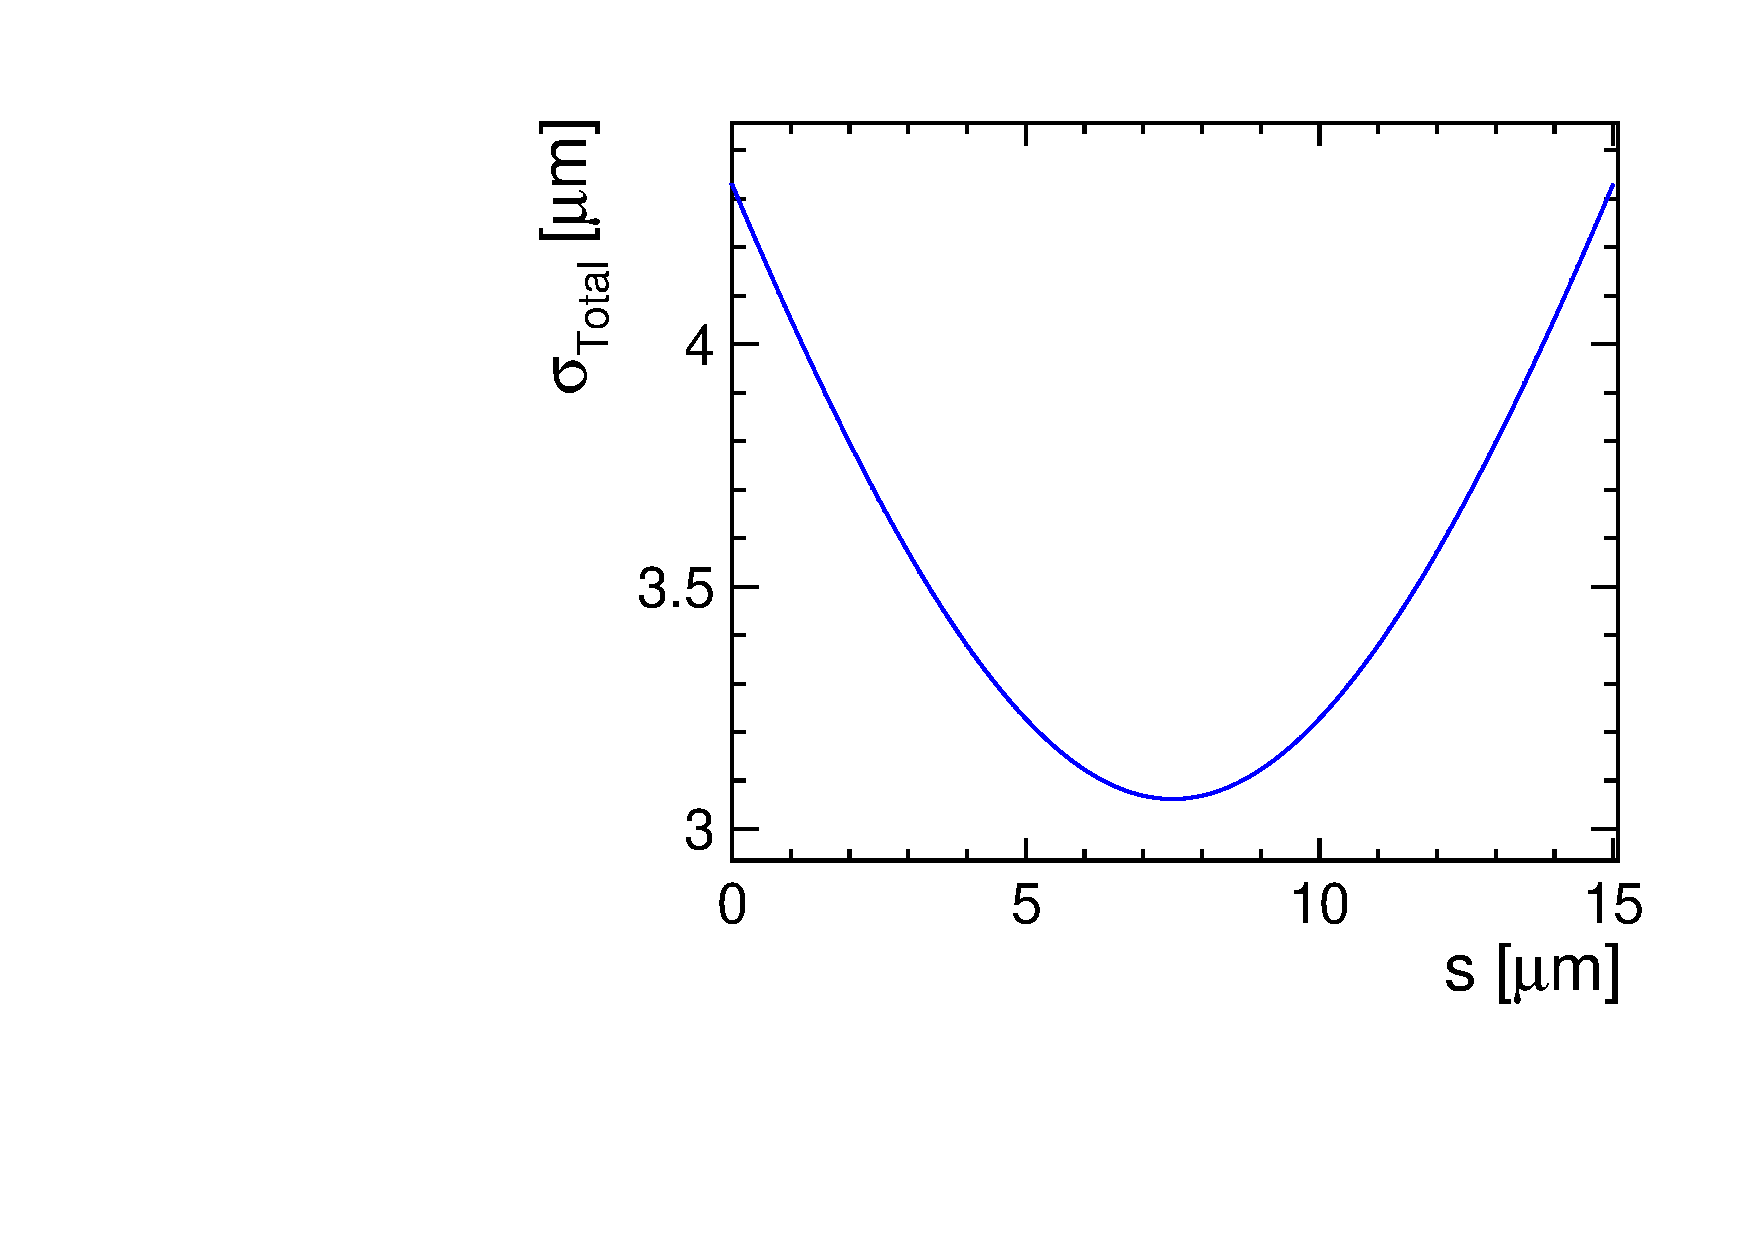
\includegraphics[width=\textwidth]{figures/ChargeSharing/resolution_binary_chargeSharing_s_15mupitch.pdf}
    \caption{$15\,\micron$ pitch}
  \end{subfigure} \hfill
  \begin{subfigure}[b]{0.3\textwidth}
    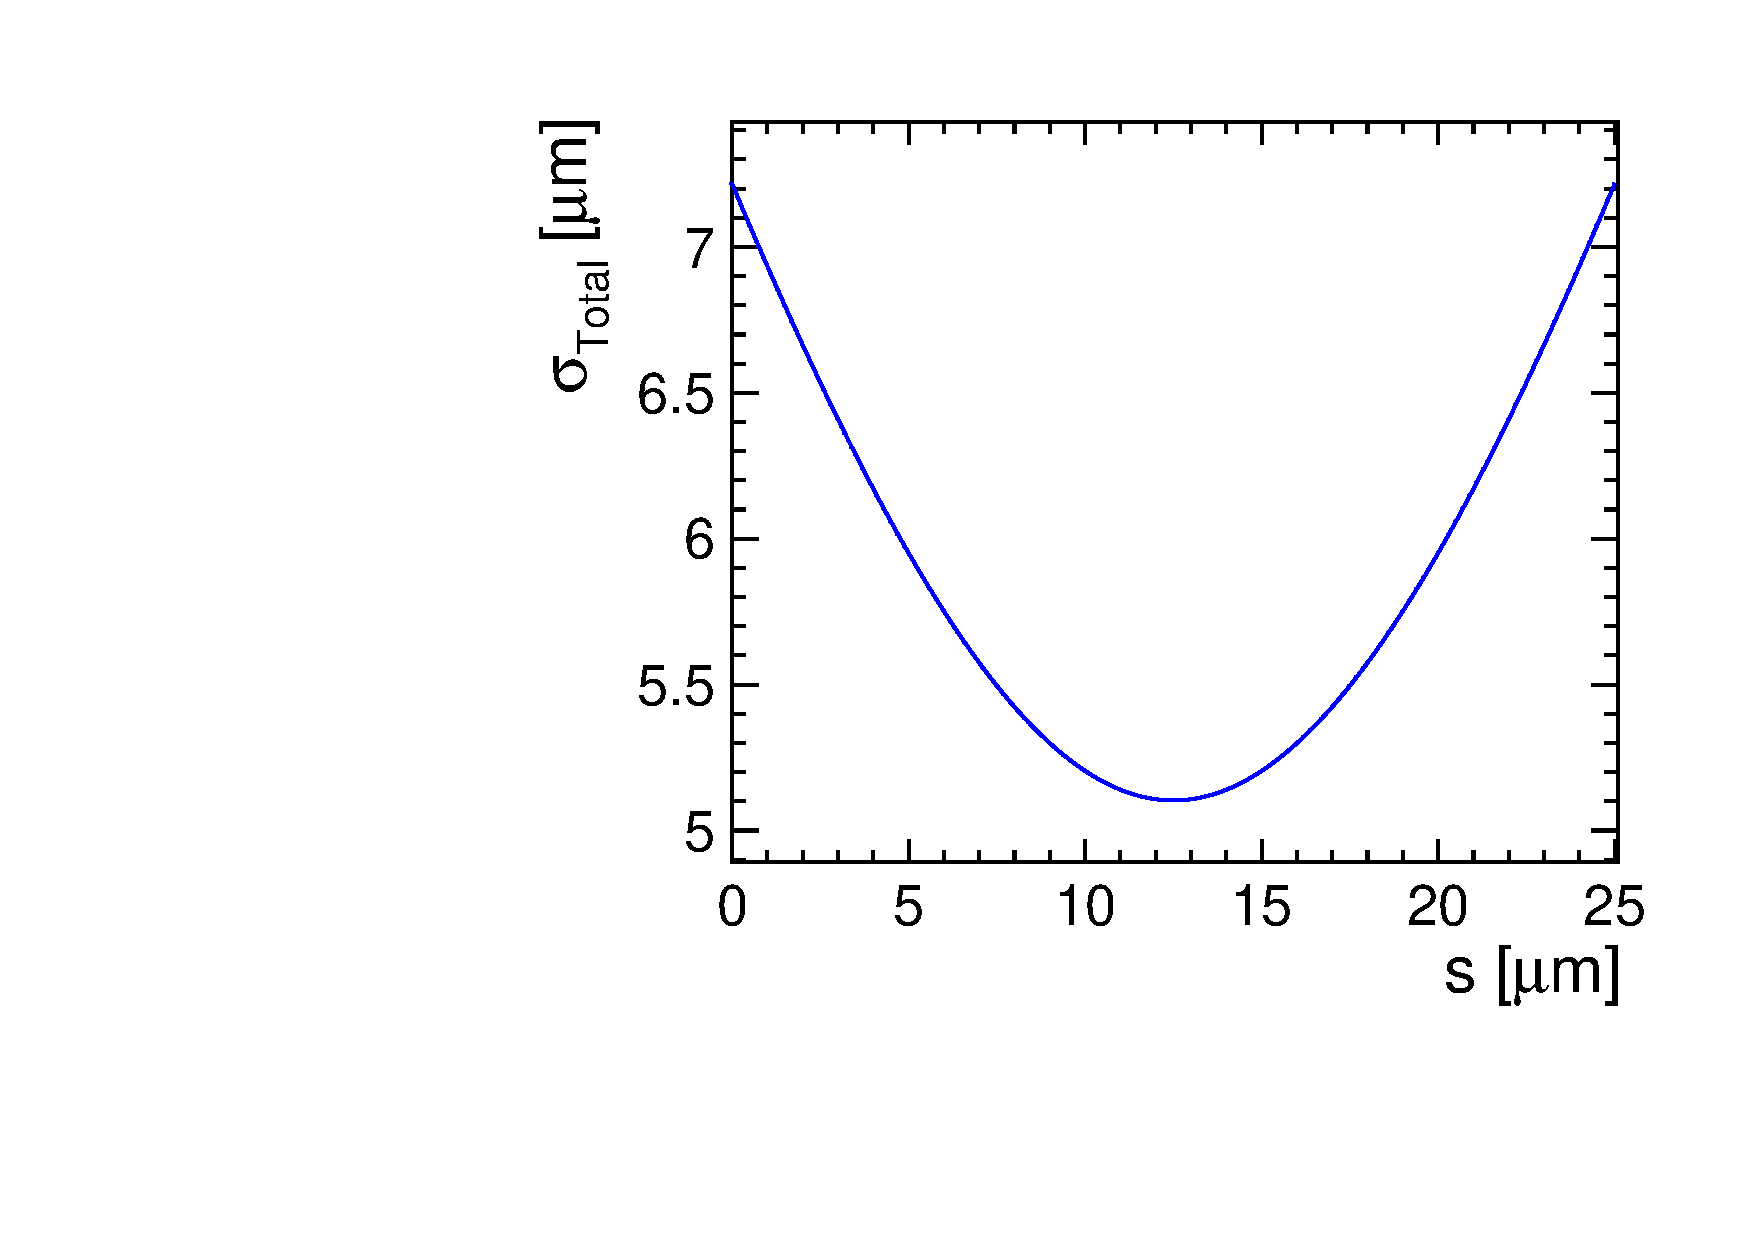
\includegraphics[width=\textwidth]{figures/ChargeSharing/resolution_binary_chargeSharing_s_25mupitch.pdf}
    \caption{$25\,\micron$ pitch}
  \end{subfigure} \hfill
  \begin{subfigure}[b]{0.3\textwidth}
    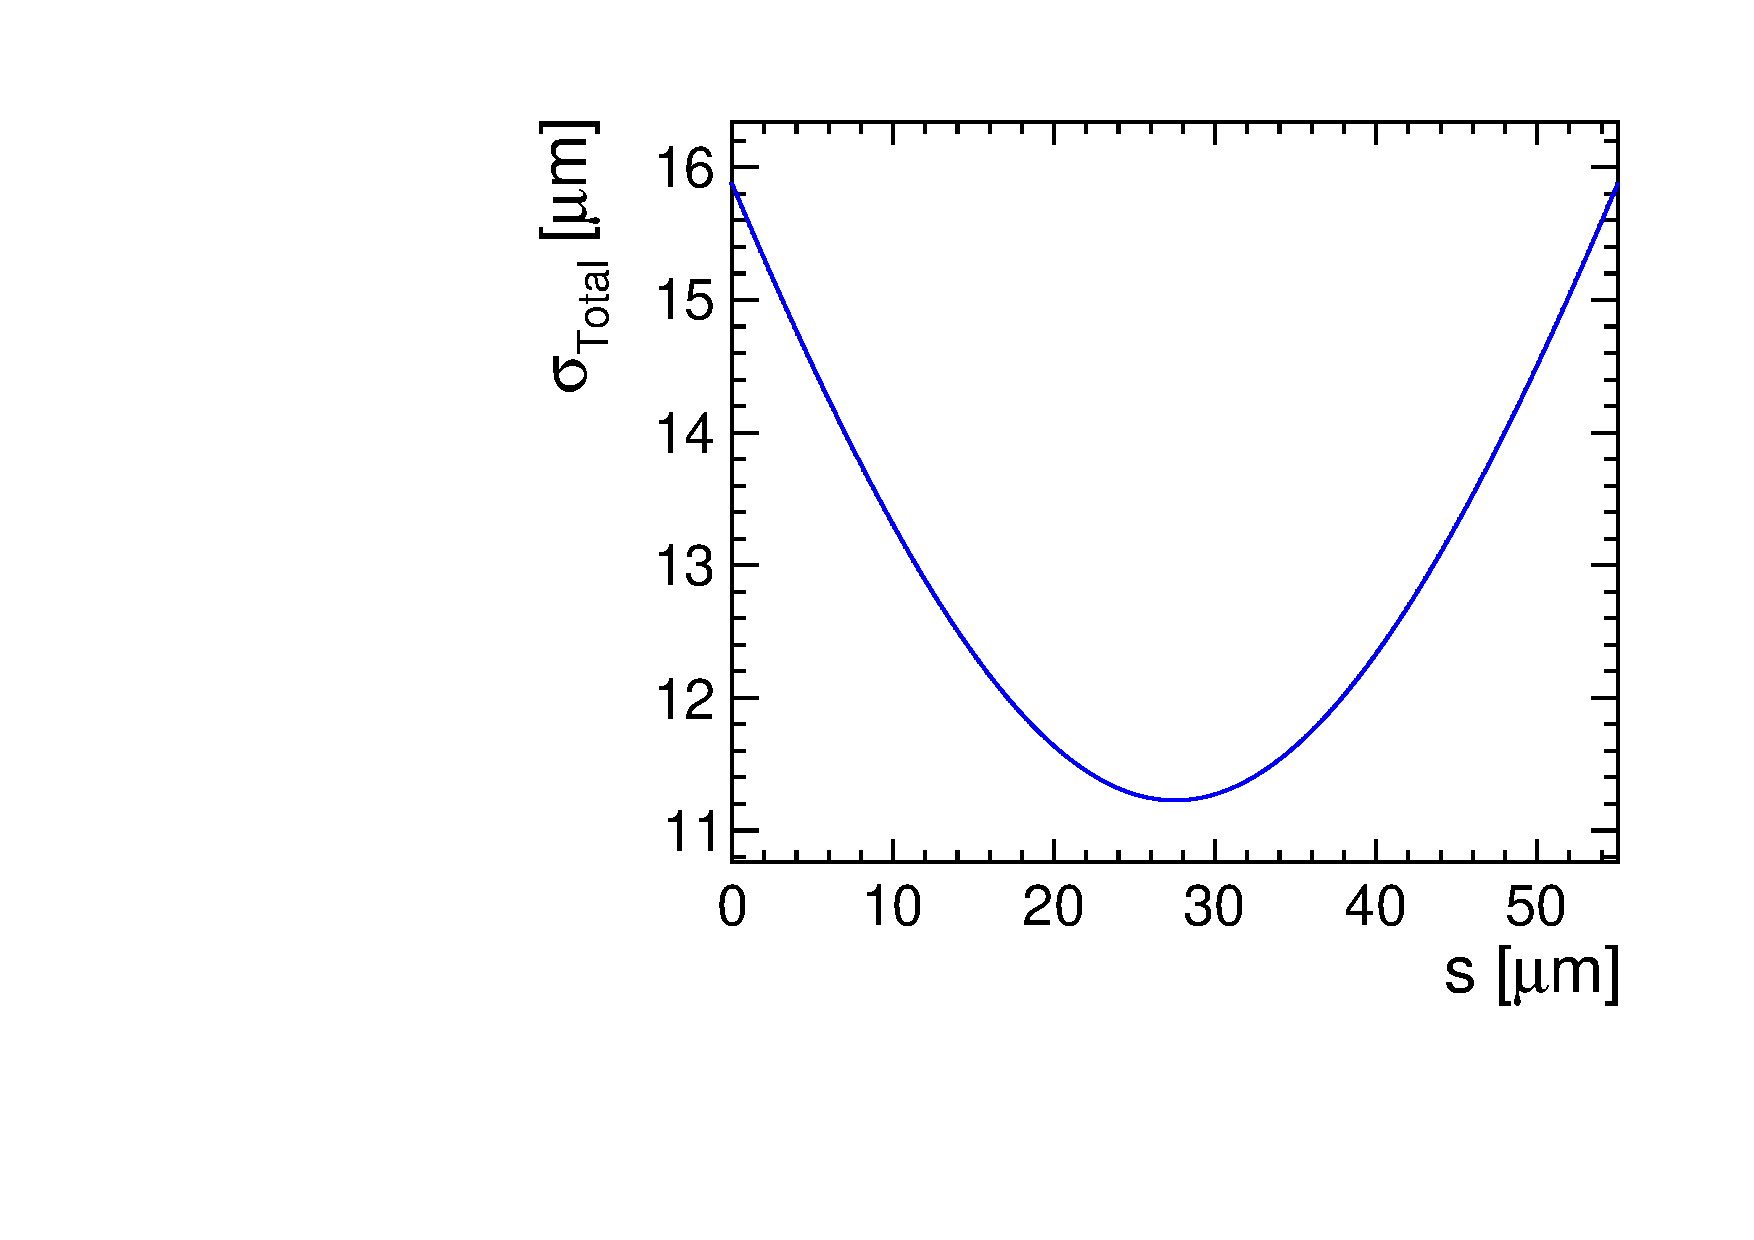
\includegraphics[width=\textwidth]{figures/ChargeSharing/resolution_binary_chargeSharing_s.pdf}
    \caption{$55\,\micron$ pitch}
  \end{subfigure}
  \caption{$\sigma_{\text{Total}}$ calculated using
    \cref{eq:spatialResChargeSharingTotal} with a pixel pitch of (a)
    $p=15\,\micron$, (b) $p=25\,\micron$ and (c) $p=55\,\micron$ where
    $s$ is the width of the charge sharing region as shown in
    \cref{fig:SpatResBinaryChargeSharing}.}
  \label{fig:sigmaTotal}
\end{figure}

%% --------------------------------------------------- %%
\subsubsection{Analogue readout and charge sharing}
\label{sec:resolutionAnalogSharing}
The spatial resolution can be significantly improved with an analogue
readout which delivers a signal proportional to the collected charge
as illustrated in \cref{fig:SpatResAnaglogChargeSharing}. In this
case, for multi-hit clusters the $\eta$-function~\cite{Belau:1983eh}
(c.f.~\cref{sec:EtaCorrection}) is used to reconstruct the hit
position within the pixels using the charge information. In the region
where only one pixel fires, the resolution is still limited to
$(p-s)\over \sqrt{12}$. Therefore the readout threshold should be as
low as possible in order to detect the smallest amounts of charge
reaching neighbouring pixels.

%% The charge carriers follow the field lines to end-up on a certain
%% electrode. They are also subject to thermal diffusion which spreads
%% the charge cloud as it drifts through the silicon. The width of the
%% diffusion $\sigma_{diffusion}(z)$ (for simplicity called $\sigma(z)$)
%% at depth $z$ is given by \cref{eq:driftTimeIntegrated}. The charge
%% distribution at position $x_{hit}$ for a pixel extending from $x_1$ to
%% $x_2$ is:
%% \begin{equation}
%% Q(x_{hit}, z)= Q(z) {1\over{\sqrt{2 \pi \sigma^2(z)}}}
%% {\int_{x_1}^{x_2} e^{-({{x-x_{hit}}\over{\sqrt{2} \sigma(z)}})^2} } dx\; .
%% \label{eq:ChargeDistribution}
%% \end{equation}

%% By integrating \cref{eq:ChargeDistribution} over the whole
%% thickness of the detector, the charge deposited in a pixel at
%% coordinate $x_{hit}$ having coordinates $x_1$ and $x_2$ is given by:  
%% \begin{equation}
%% Q(x_{hit})= \int_{x_1}^{x_2}  \int_{0}^{d} {Q(z) \over {\sqrt{2 \pi
%%       \sigma^2(z)}} } e^{-({{x-x_{hit}}\over{\sqrt{2} \sigma(z)}})^2}
%%   dz \; dx\; .
%% \label{eq:ChargeDistribution_integrated_z}
%% \end{equation}


\begin{figure}[htbp]
  \centering
  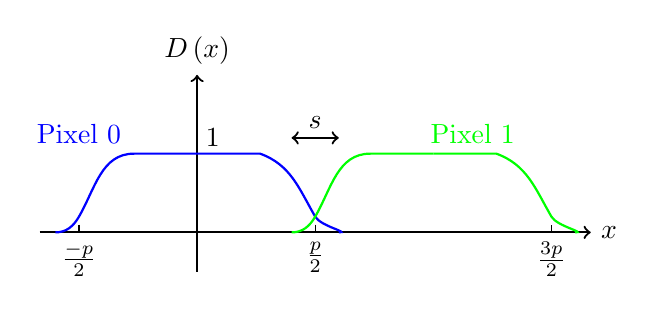
\begin{tikzpicture}
    \begin{scope}
      
      \draw[->, thick] (-2,0)--(5,0) node[right]{$x$};
      \draw[->, thick] (0, -0.5)--(0, 2) node[above]{$D\left(x\right)$};
      
      \draw[thick, blue] (-1.8,0) to[out=0, in=-120] (-1.5,0.2) to[out=60, in=180](-0.8, 1)--(0,1);
      \draw[thick, blue] (0,1)--(0.8, 1) to [out=-20, in=120] (1.5, 0.2) to[out=-60, in=0] (1.8,0);

      \draw[-] (-1.5, 0.1) -- (-1.5, 0) node[below] {${-p \over 2}$};
      \draw[-] (1.5, 0.1) -- (1.5, 0) node[below] {${p \over 2}$};
      \node[above, blue] at (-1.5, 1) {Pixel 0};

      \node[] at (0.2, 1.2) {1};


      \draw[thick, green] (1.2,0) to[out=0, in=-120] (1.5,0.2) to[out=60, in=180](2.2, 1)--(3,1);
      \draw[thick, green] (3,1)--(3.8, 1) to [out=-20, in=120] (4.5, 0.2) to[out=-60, in=0] (4.8,0);
      \draw[-] (4.5, 0) -- (4.5, 0.1);
      \node[below] at (4.5, 0) {${{3p} \over 2}$};
      \node[above, green] at (3.5, 1) {Pixel 1};

      \draw[<->, thick] (1.2, 1.2)--(1.8, 1.2);
      \node[above] at (1.5, 1.2) {$s$}; 
    \end{scope}
  \end{tikzpicture}
  \caption{The hit probability density function for two neighbouring
    pixels (pixel 0 and pixel 1) considering charge sharing between
    the two pixels using an analogue to acquire the sensor
    pulse.}\label{fig:SpatResAnaglogChargeSharing}
\end{figure}

%% --------------------------------------------------- %%
\section{The $\eta$-correction method}
\label{sec:EtaCorrection}

Due to the charge sharing, particle tracks create multi-pixel
clusters. The hit position within the pixel is reconstructed by using
the charges of the hit pixels as weights. The method also takes into
account non-linearities in the charge sharing between
pixels~\cite{Belau:1983eh}.

The $\eta$-correction method calculates the distance with which the
hit position moves from the geometric centre of two pixels in a
cluster.

\begin{equation}
  \text{shift}=\sigma_{EC} \times \text{erf}^{-1}(2\times Q_{rel}-1) \; ,
  \label{eq:EtaCorrectionShift}
\end{equation}

where $\sigma_{EC}$ is a parameter to be determined and depends on
several factors such as the thickness of the silicon sensor and the
operating conditions of the assembly. The inverse error function is
defined as erf\textsuperscript{-1} (z) with:

\begin{equation}
\text{erf(z)}={2\over\sqrt{\pi}} \int_{0}^{z} e^{-t^2} dt \; .
  \label{eq:EtaCorrectionErf}
\end{equation}

In \cref{eq:EtaCorrectionShift}, $Q_{rel}$ is the maximum charge of
the cluster divided by the total charge of the cluster
($Q_{max}/Q_{tot}$).


%% --------- Recycle text --------- %%
% \section{Detector systems}

% Figure~\ref{fig:basicDetectorFunction}, schematically summarises the sequence of basic detector functions.


% \begin{figure}[htbp]
%   \centering
%   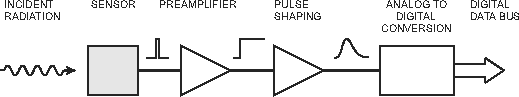
\includegraphics[width=\textwidth]{figures/basicDetectorFunction.png}
%   \caption{The sequence of basic detector functions. From~\cite{Spieler2005}.}
%   \label{fig:basicDetectorFunction}
% \end{figure}


% \subsection{Sensor} 
% A silicon sensor, converts the energy deposited by a particle to an electric signal by producing electron-hole pairs. By applying an electric field to the sensor, the produced pairs are con
% \subsection{Preamplifier}
% \subsection{Pulse shaper}
% \subsection{Digitiser}

%% --------------------------------------------------- %%
% Carriers move in random direction due to the thermal energy. \\
% Material-dependent diffusion constant given by the Einstein equation:  

% \begin{equation}
%   D_{b}={{k_{B} \cdot T \cdot \mu_{c}} \over {e}}
% \end{equation}
% where \(k=8.617 3324\) is the Boltzman constant.

% \begin{equation}
%   \sigma_{diffusion}=\sqrt{2 \cdot D_{b} \cdot t_{c}}
% \end{equation}






%% \begin{table}[htpb]
%%   \centering
%%   \caption{Sensors characteristics:}
%%   \label{tab:Efield_mobility}
%%   \begin{tabular}{ c c c c c c }
%%     \toprule
%%     Assembly & Sensor type & Thickness & V\textsubscript{depletion} &  V\textsubscript{bias} & THL\textsubscript{op} \\
%%     \midrule
%%     A06-W0110 & p-in-n & 50~\micron & $<15$~V & 15~V & 326 (855e\textsuperscript{-}) \\
%%     L04-W0125 & p-in-n & 100~\micron & 19.64~V & 35~V & 410 (916e\textsuperscript{-}) \\
%%     B06-W0125 & n-in-p & 200~\micron  & 30.31~V & -50~V & 435 (1066e\textsuperscript{-}) \\
%%     \bottomrule
%%   \end{tabular}
%% \end{table}

%% \begin{figure}[htbp]
%%   \centering
%%   \begin{subfigure}[b]{0.33\textwidth}
%%     \centering
%%     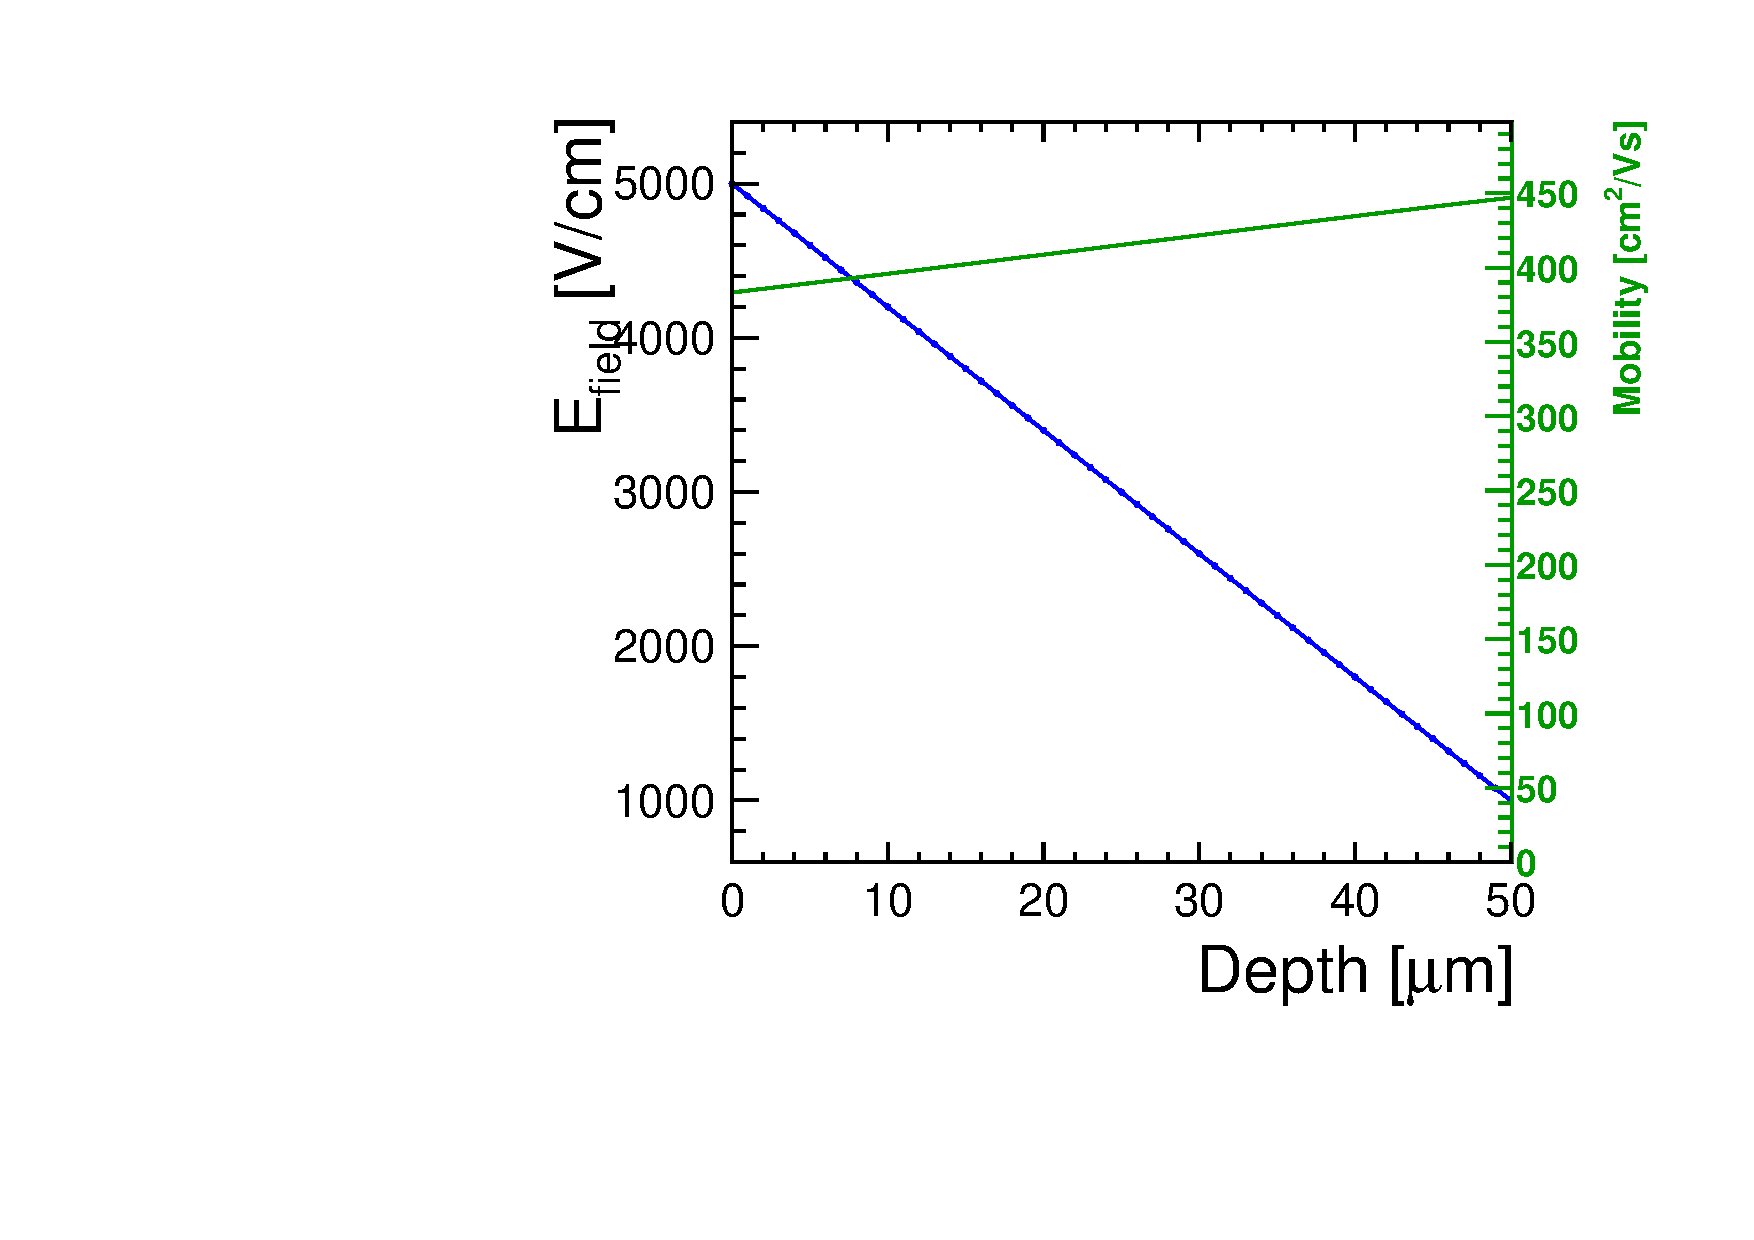
\includegraphics[width=\textwidth]{figures/ChargeSharing/Efield_mob_A06.pdf}
%%     \caption{50~\micron silicon}\label{fig:Mob_Efield_A06}
%%   \end{subfigure}\hfill
%%   \begin{subfigure}[b]{0.33\textwidth}
%%     \centering
%%     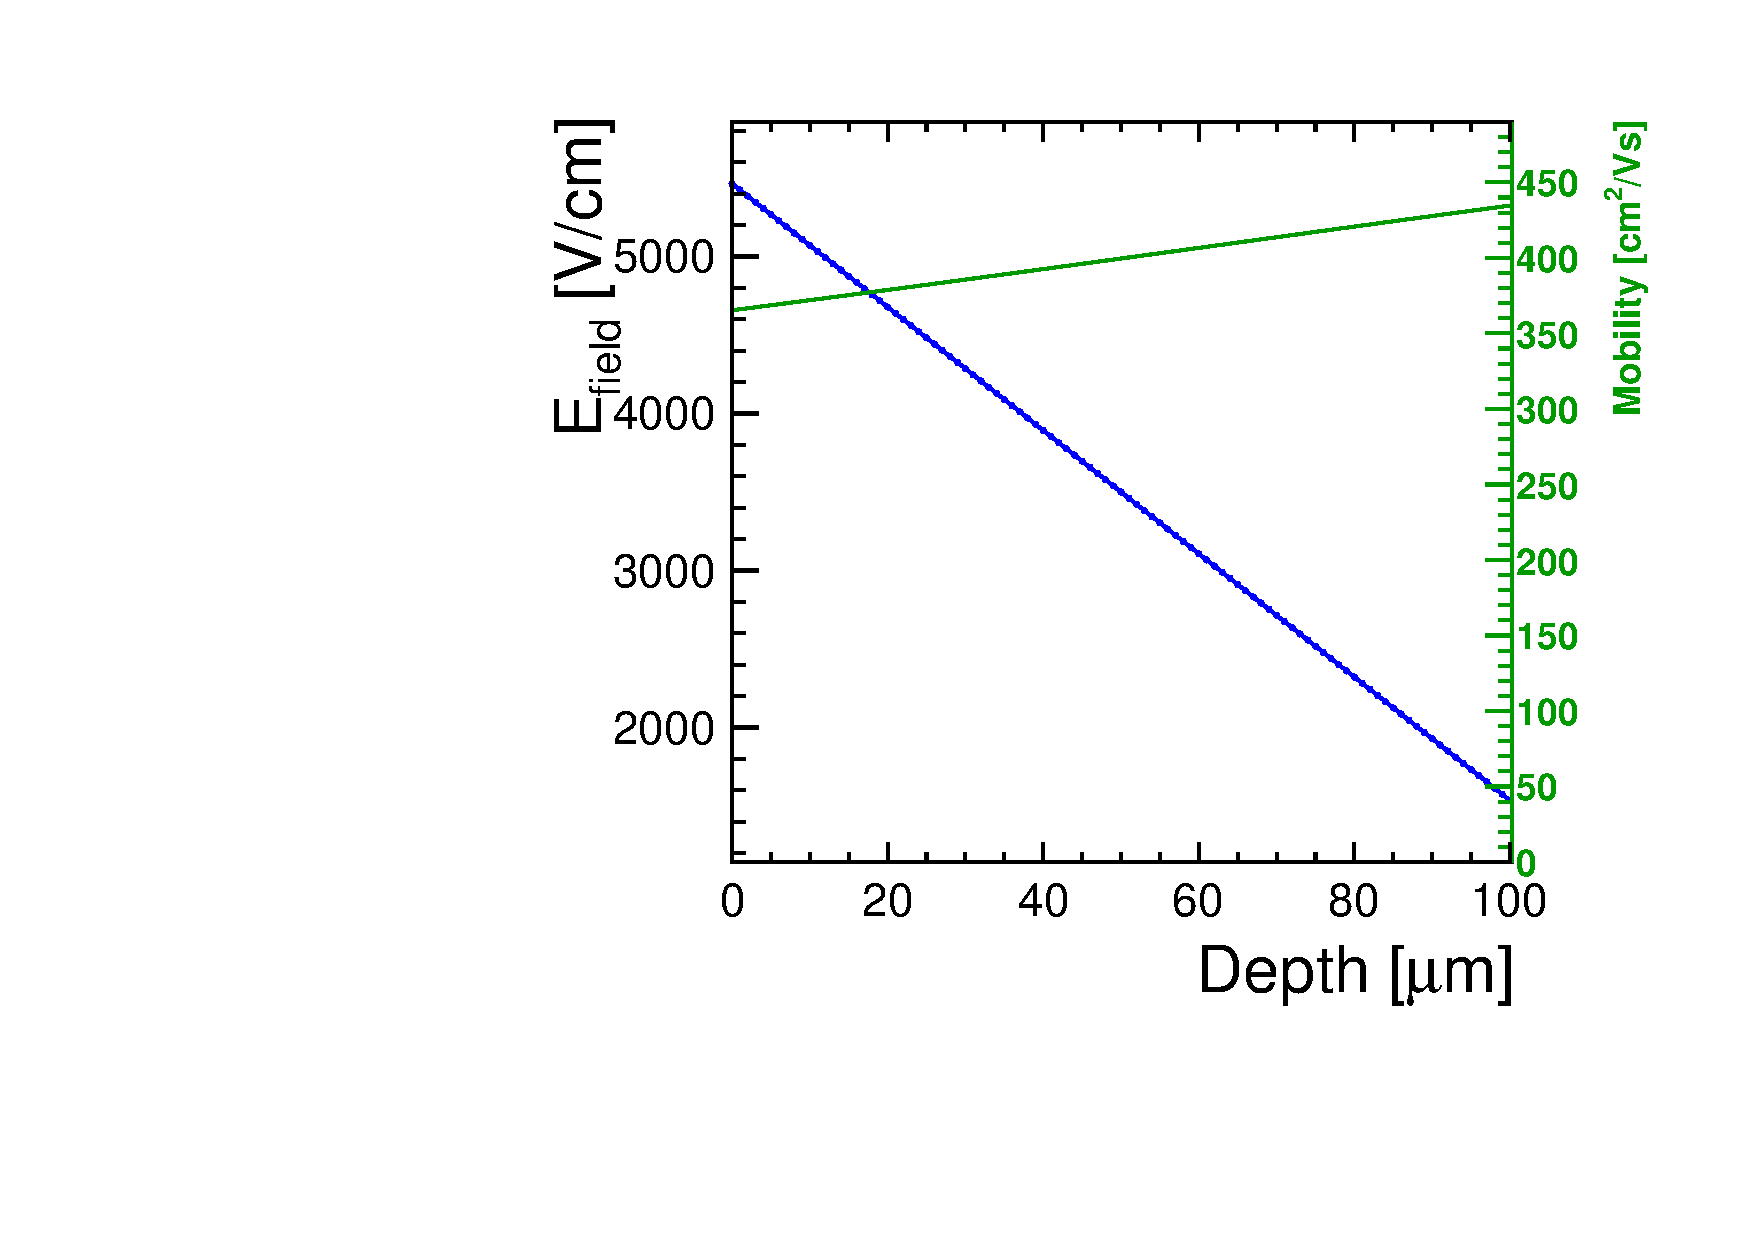
\includegraphics[width=\textwidth]{figures/ChargeSharing/Efield_mob_L04.pdf}
%%     \caption{100~\micron Silicon}\label{fig:Mob_Efield_L04}
%%   \end{subfigure} \hfill
%%   \begin{subfigure}[b]{0.33\textwidth}
%%     \centering
%%     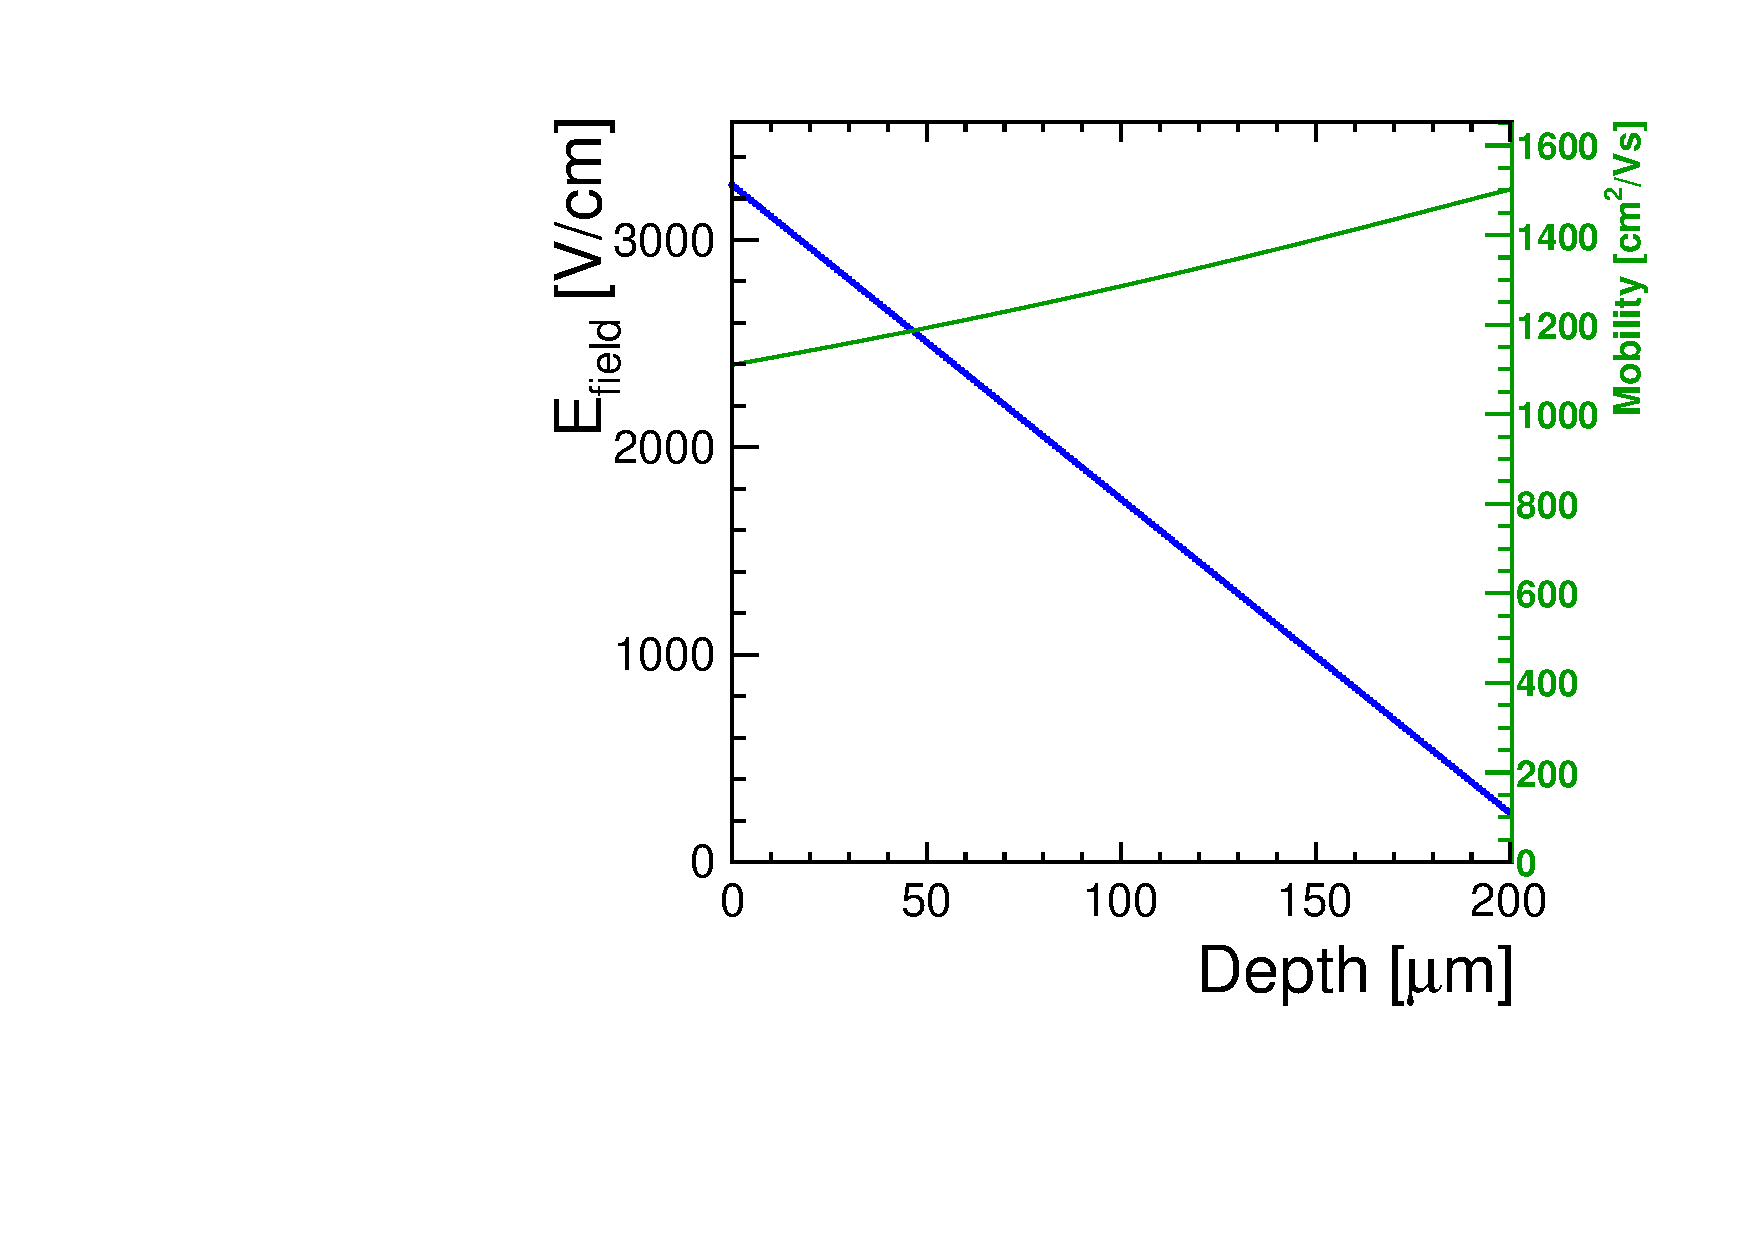
\includegraphics[width=\textwidth]{figures/ChargeSharing/Efield_mob_B06.pdf}
%%     \caption{200~\micron Silicon}\label{fig:Mob_Efield_B06}
%%   \end{subfigure} 
%%   \caption{Mobility dependence on the electric field.}\label{fig:Efield_mobility}
%% \end{figure}

%% Assuming the mobility constant is a good approximation for calculating
%% the charge sharing spread since the electric field is low. An example
%% is given for the case where the silicon sensor has a thickness of 200~\micron.

%% \begin{figure}[htbp]
%%   \centering
%%   \begin{subfigure}[b]{0.49\textwidth}
%%     \centering
%%     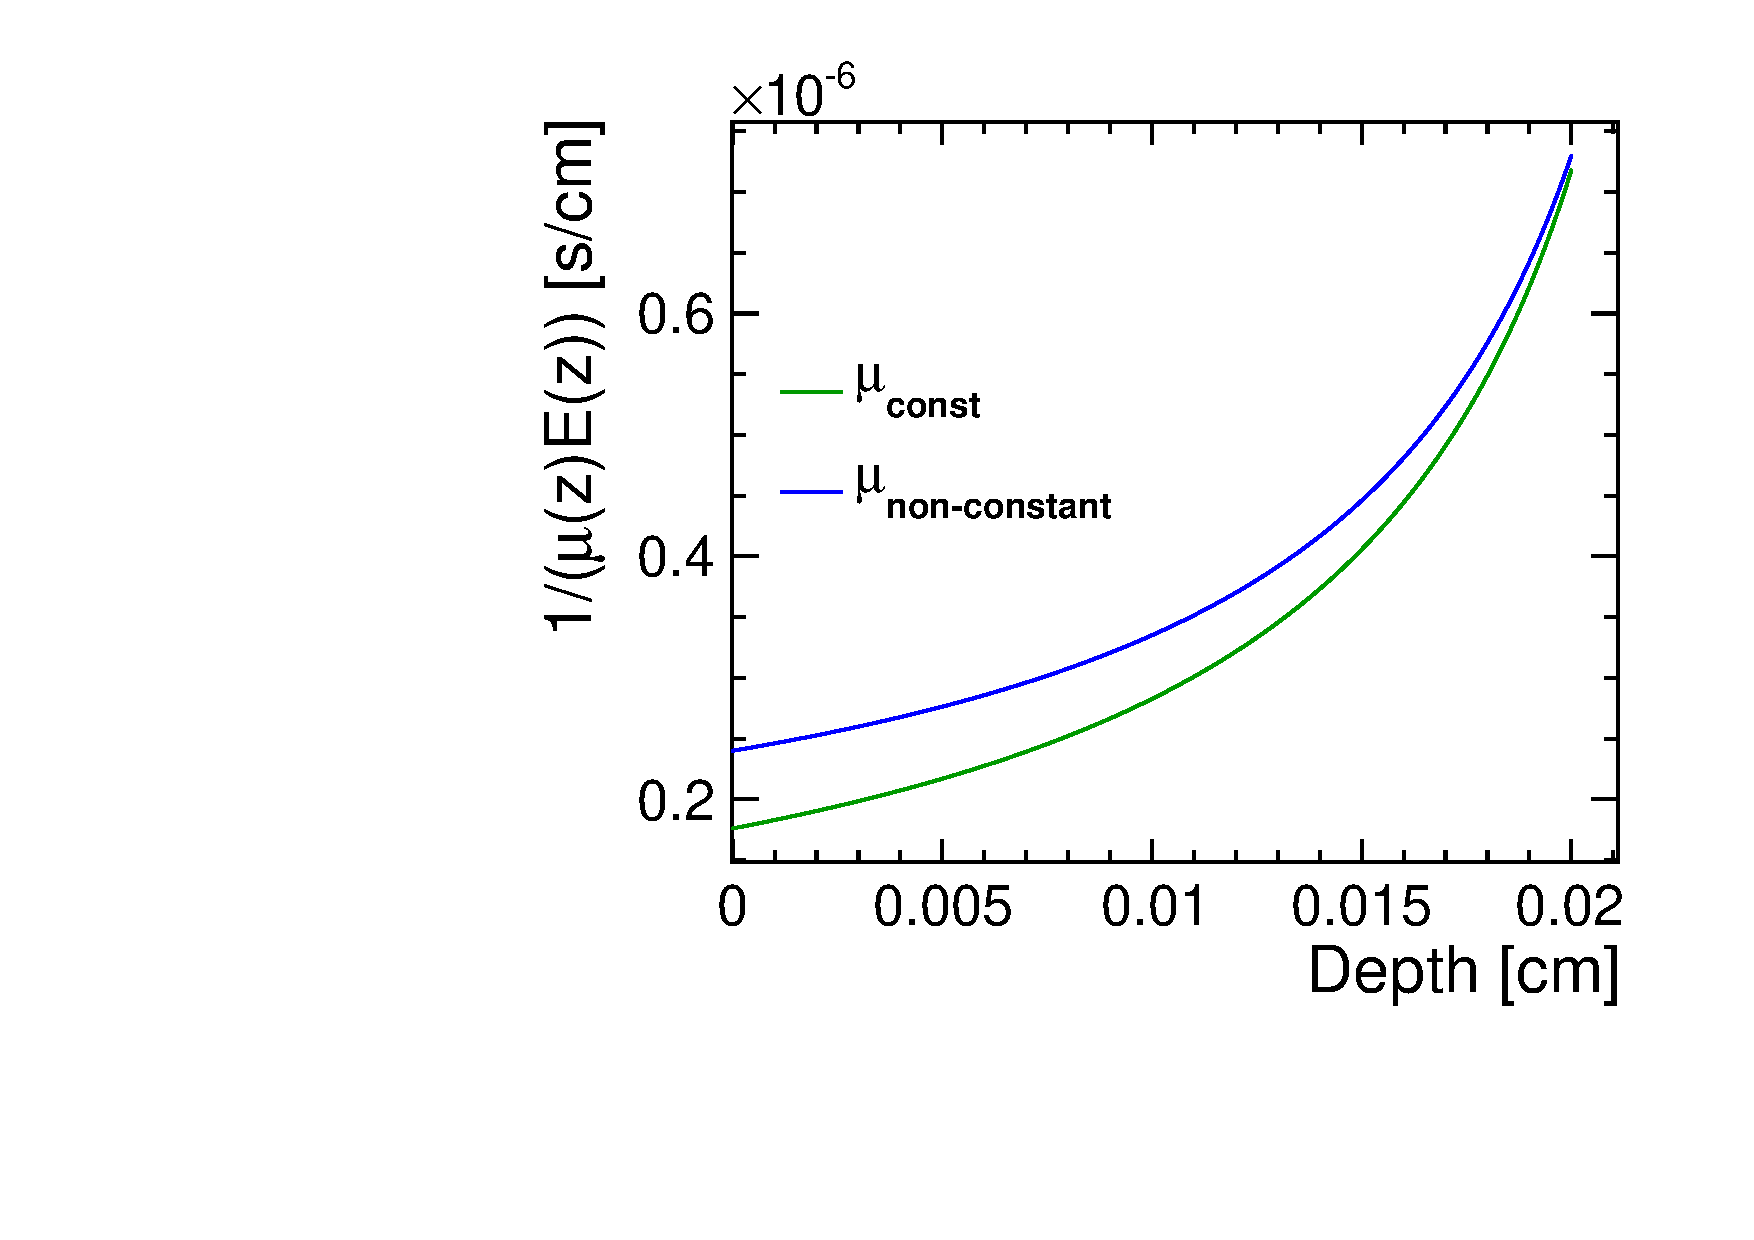
\includegraphics[width=\textwidth]{figures/ChargeSharing/B06_FunctionToIntegrate.pdf}
%%     \caption{}\label{fig:}
%%   \end{subfigure}\hfill
%%   \begin{subfigure}[b]{0.49\textwidth}
%%     \centering
%%     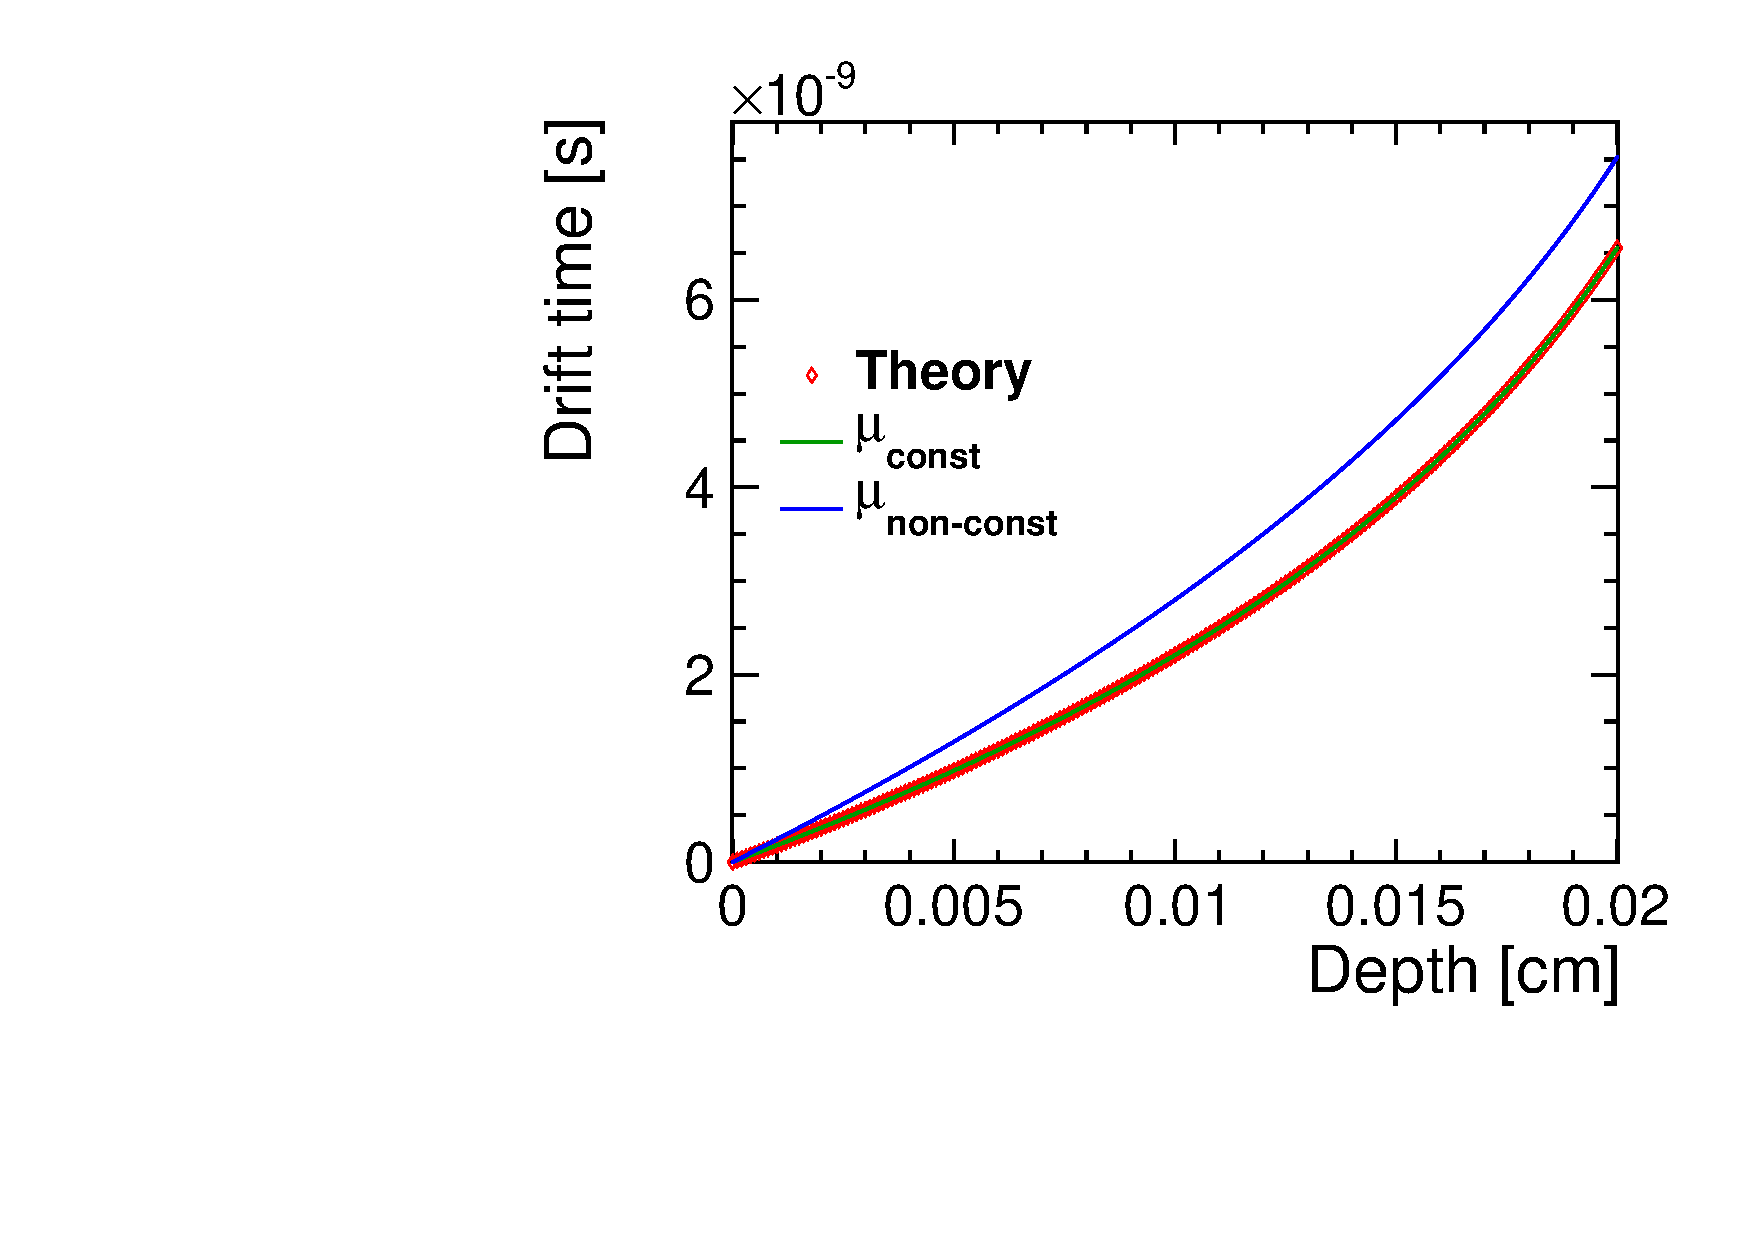
\includegraphics[width=\textwidth]{figures/ChargeSharing/B06_driftTime.pdf}
%%     \caption{}\label{fig:}
%%   \end{subfigure} 
%%   \caption{Drift time considering the mobility constant or non-constant.}\label{fig:}
%% \end{figure}

%% The diffusion constant and the diffusion spread considering the
%% mobility constant and non-constant.
%% \begin{figure}[htbp]
%%   \centering
%%   \begin{subfigure}[b]{0.49\textwidth}
%%     \centering
%%     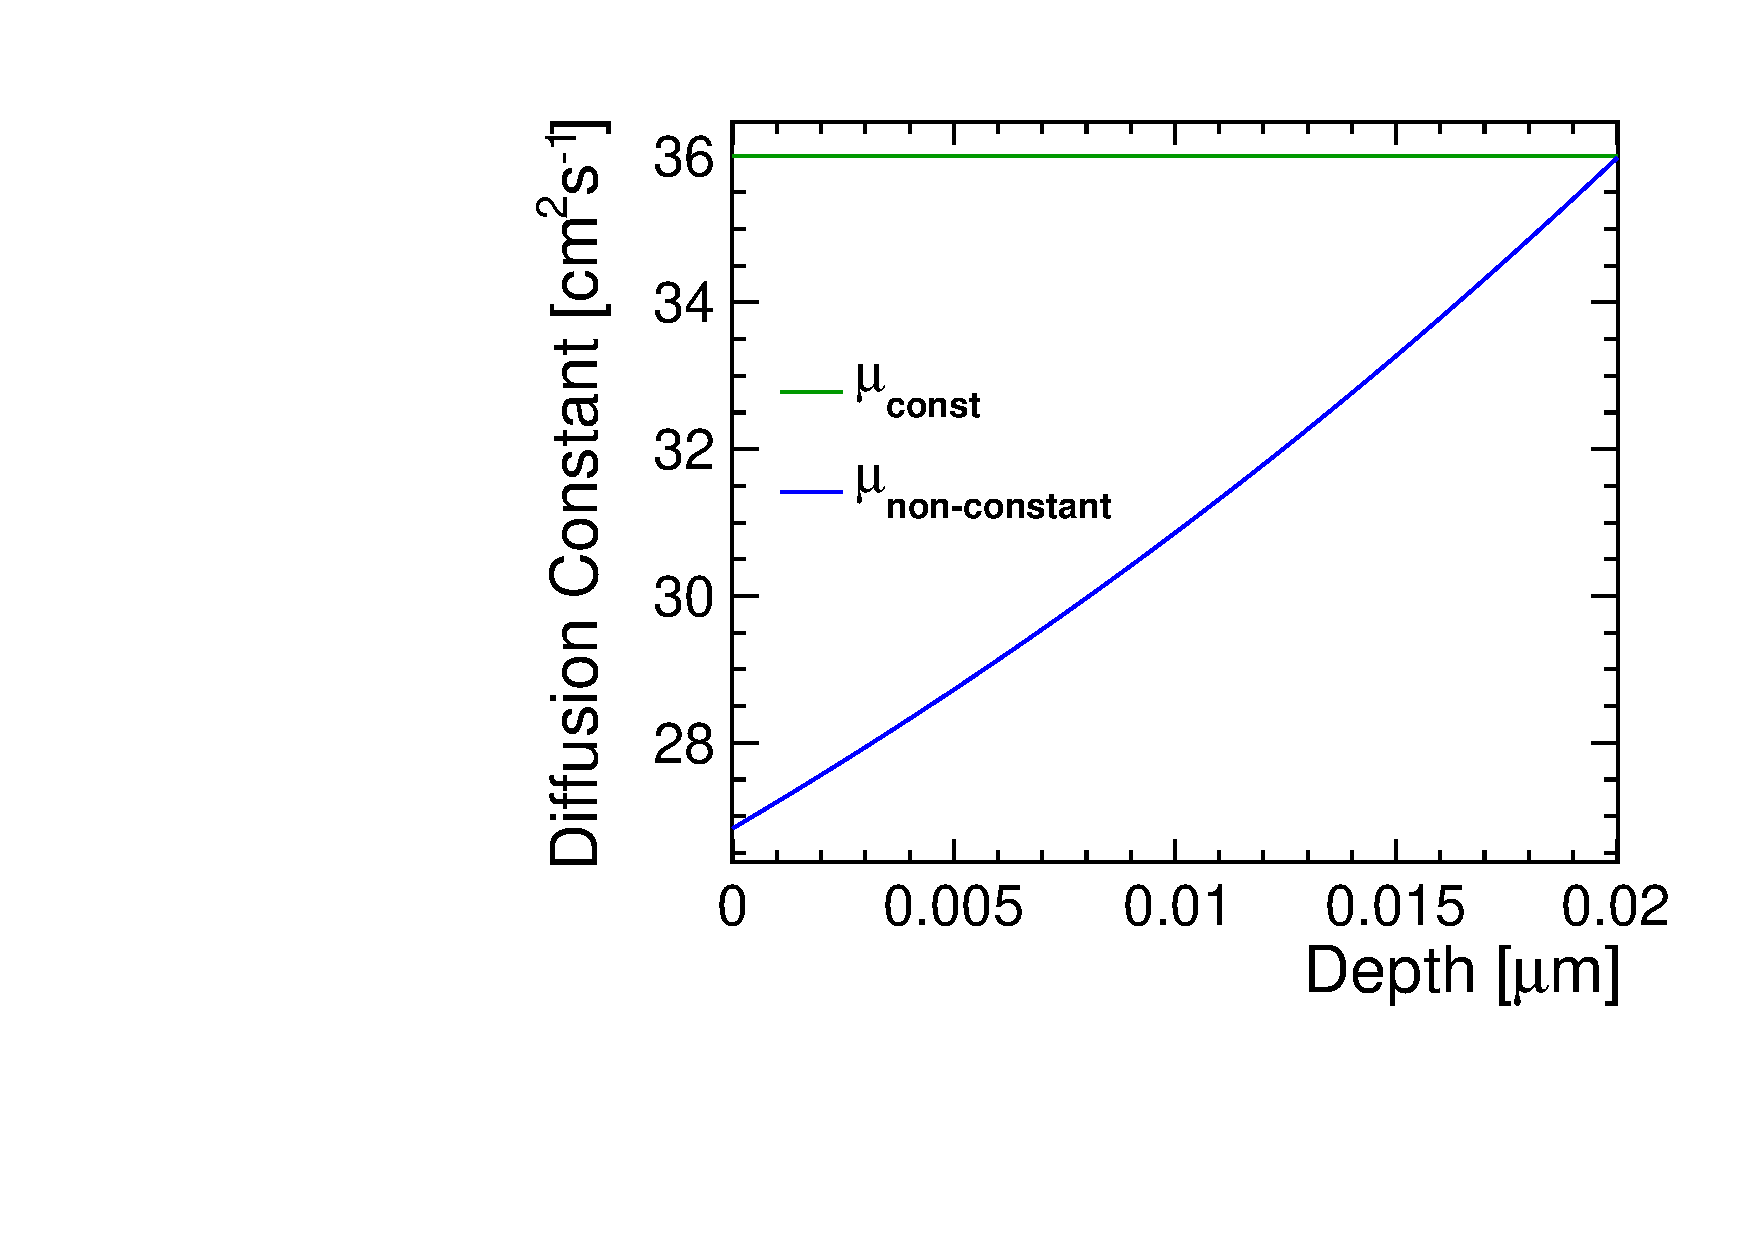
\includegraphics[width=\textwidth]{figures/ChargeSharing/B06_DiffusionConstant.pdf}
%%     \caption{}\label{fig:}
%%   \end{subfigure}\hfill
%%   \begin{subfigure}[b]{0.49\textwidth}
%%     \centering
%%     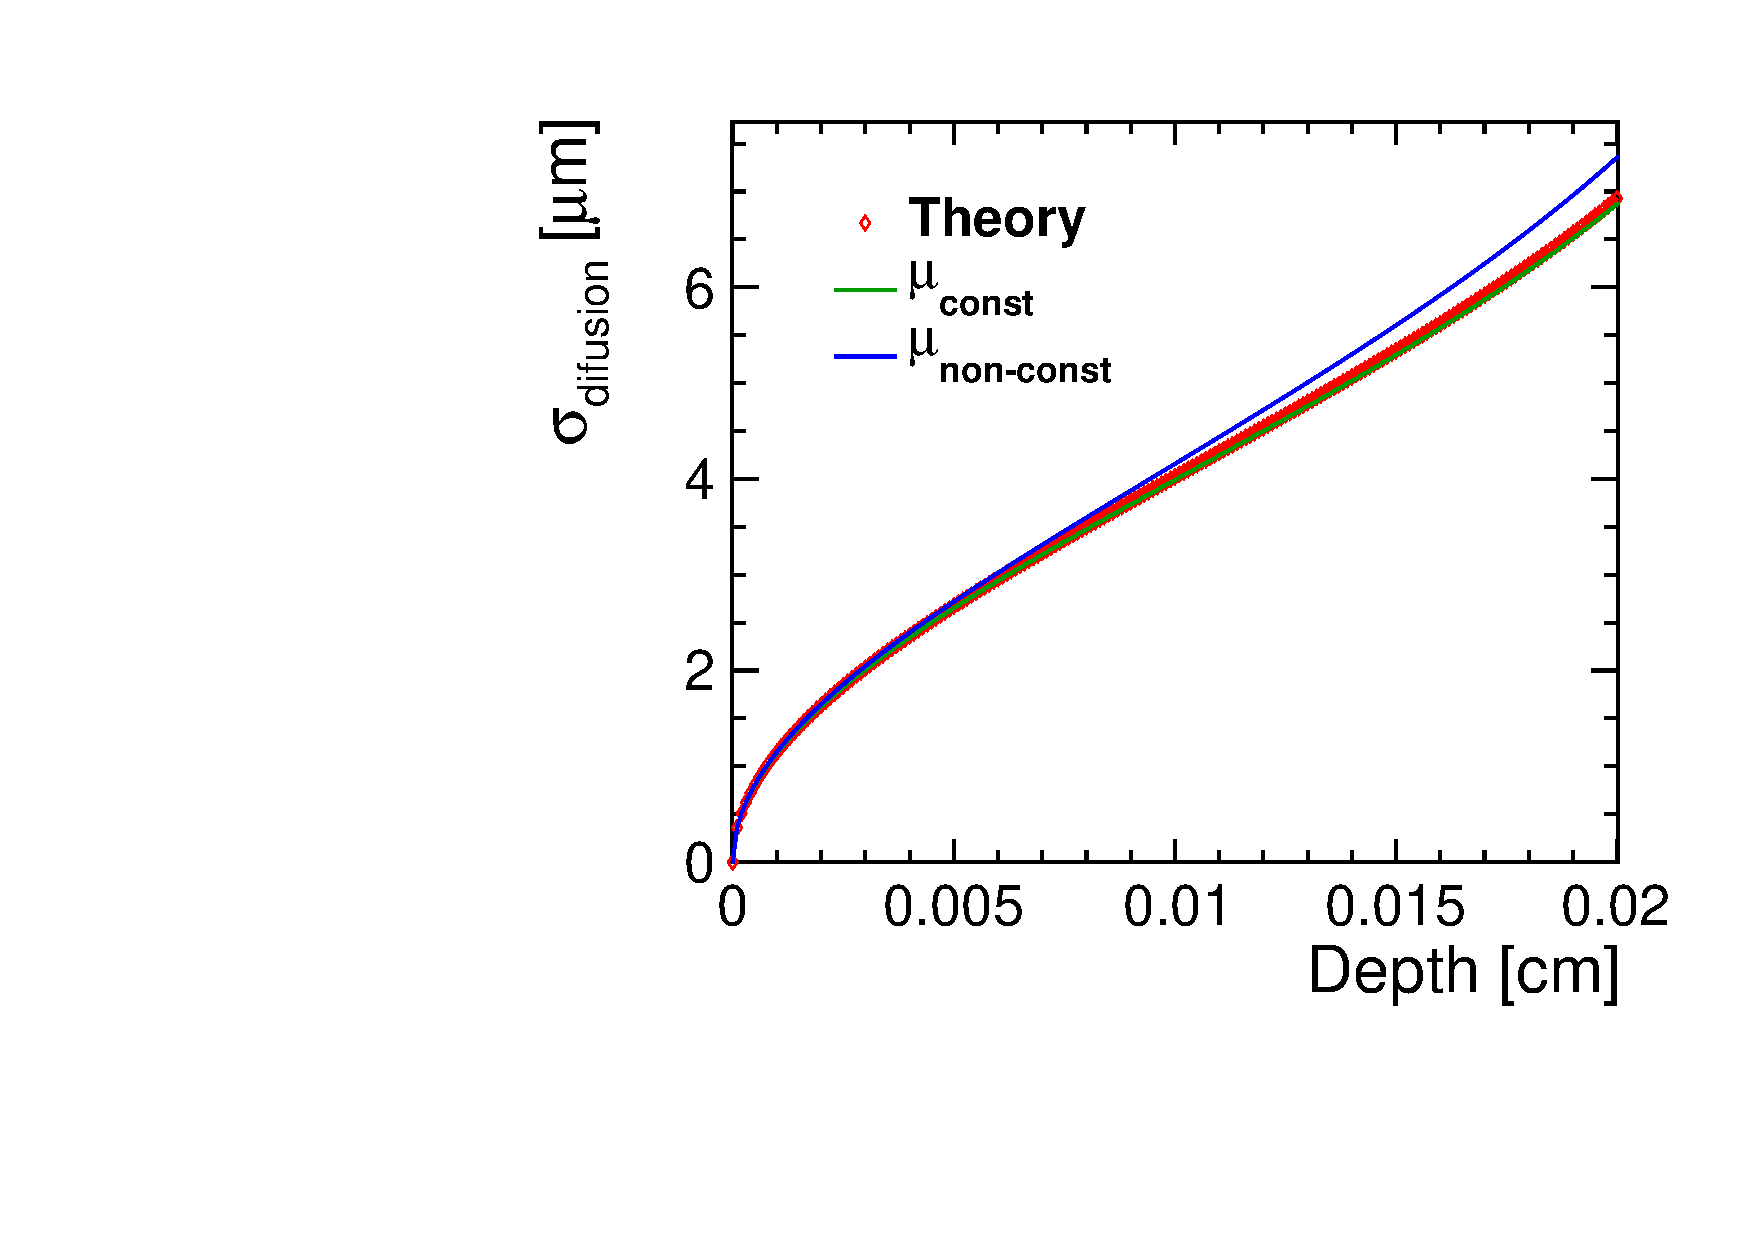
\includegraphics[width=\textwidth]{figures/ChargeSharing/B06_SigmaDiffusion.pdf}
%%     \caption{}\label{fig:}
%%   \end{subfigure} 
%%   \caption{The diffusion constant and spread for a constant mobility
%%     and a mobility which depends on the electric field. }\label{fig:}
%% \end{figure}

%% Comparing TCAD simulations and the charge sharing obtained by the
%% theoretical calculations gives us the following for a 200~\micron with
%% a depletion voltage of 30.31~V. Comparing for two different bias
%% voltages of 35~V and 50~V. In the case of the TCAD
%% simulations these results depend largely on the mesh divisions and
%% their locations. Both TCAD and theory assume a charge deposition of
%% 80e- per \micron.

%% \begin{figure}[htbp]
%%   \centering
%%   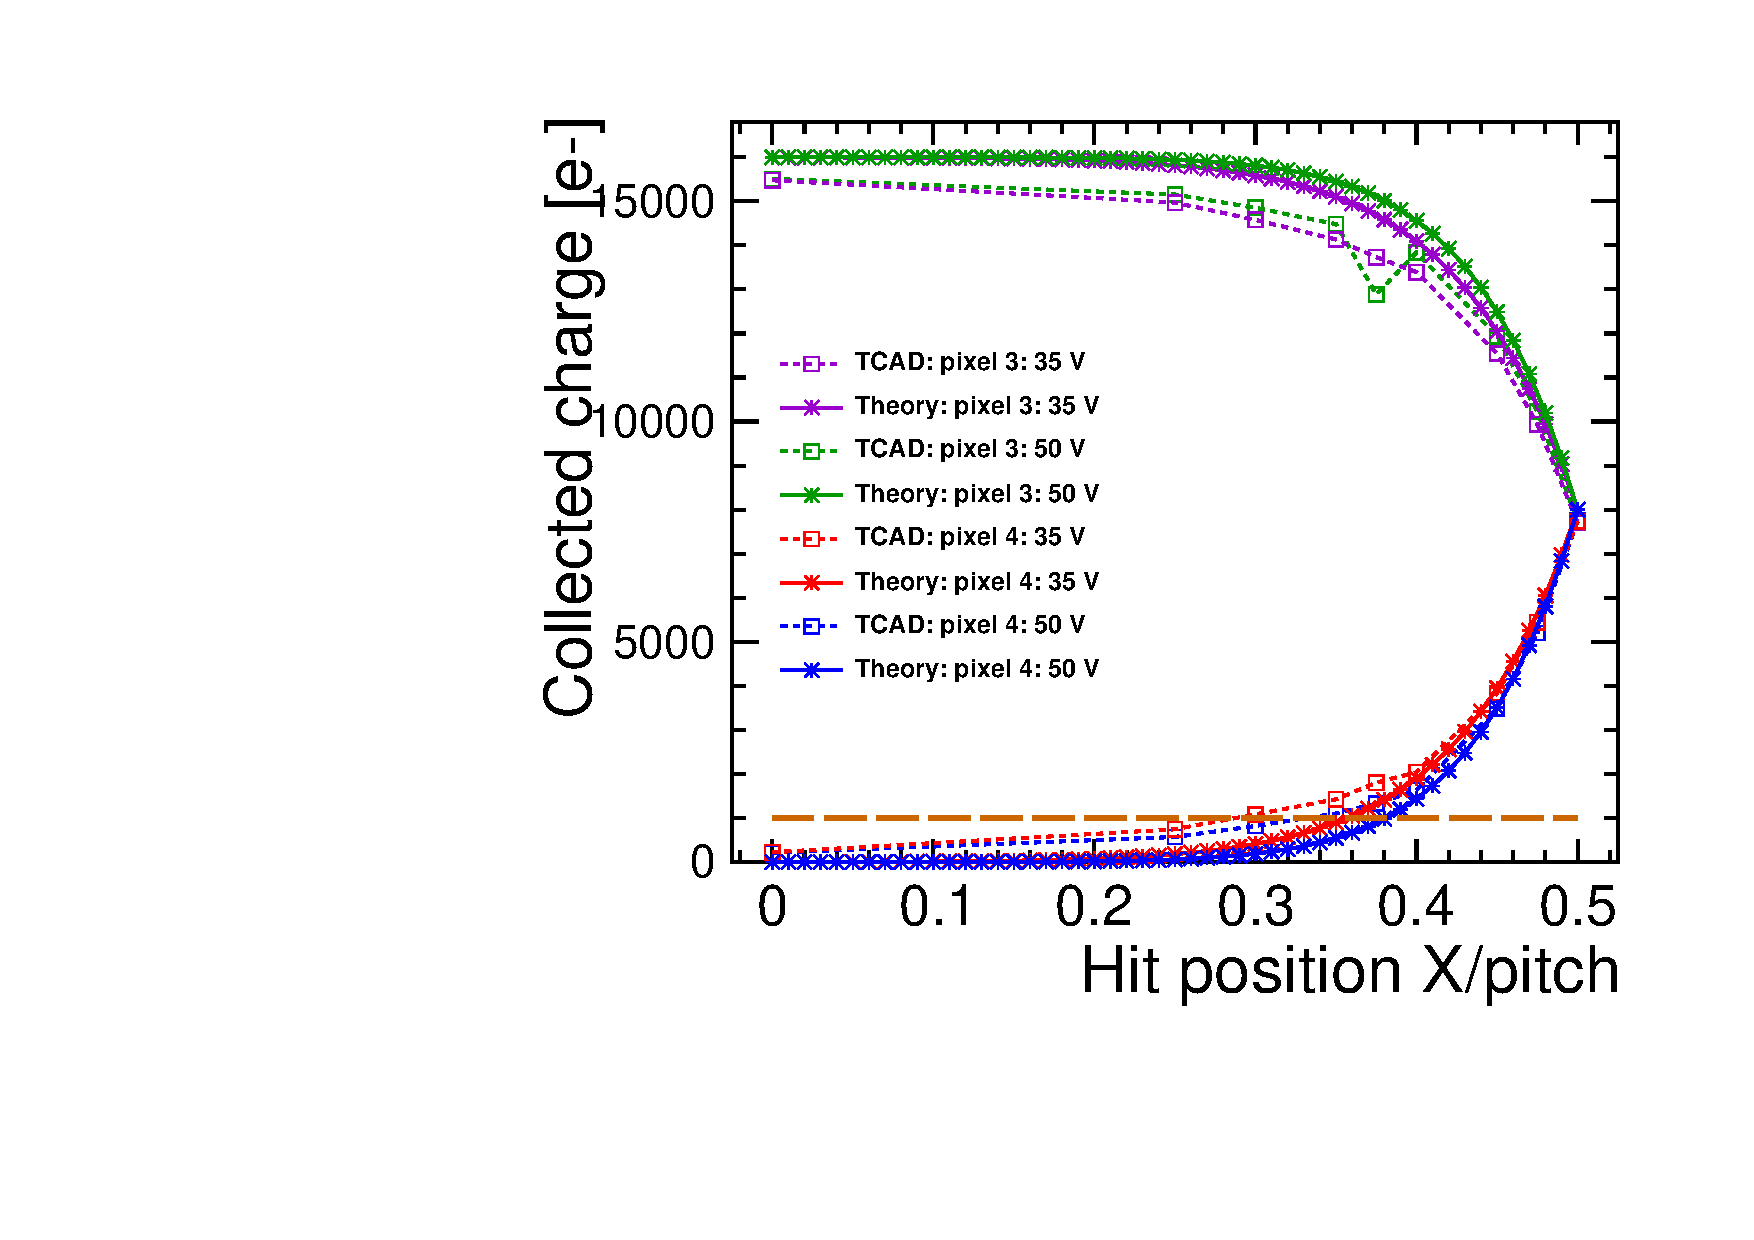
\includegraphics[width=0.5\textwidth]{figures/ChargeSharing/tcad_vs_theory.pdf}
%%   \caption{Diffusion comparing TCAD and theory.}\label{fig:}
%% \end{figure}
